\label{sec:bldata}

To reduce turbulence-driven uncertainty in aerothermodynamic heating predictions
for blunt-bodied reentry vehicles, new direct numerical simulations of
spatiotemporally homogenized boundary layers were performed to address the need
for high-quality turbulence model calibration data identified in
\autoref{sec:review}.
%
In this chapter, the characteristics of these new homogenized boundary layer
simulations are examined.
%
The chapter additionally provides enough information so that a
prediction-oriented practitioner may assess this new data's merit towards
inclusion in some calibration process.
%
The simulations will be described and analyzed, which includes
simulation details (\autoref{sec:bldata_details}), notes on the observed
integral boundary layer thicknesses (\autoref{sec:bldata_integrallengths}), turbulence
statistics (\autoref{sec:bldata_stats}), and Favre-averaged equation budgets
(\autoref{sec:bldata_budgets}).

For a more in-depth investigation of the homogenization see
\citet{Topalian2014Spatiotemporal}.
%
Also note that homogenization-related forcing terms from that reference must
be incorporated when calibrating a turbulence model using the present results.
The terms are not, however, required for subsequent use of a calibrated model.


%%%%%%%%%%%%%%%%%%%%%%%%%%%%%%%%%%%%%%%%%%%%%%%%%%%%%%%%%%%%%%%%%%%%%%%%%%%%%%
\section{Simulation Details}
\label{sec:bldata_details}

Two cold-wall boundary layers were simulated at conditions representative of
flow over the Orion MPCV thermal protection system at peak heating during
vehicle reentry from the International Space Station.
%
Additional background on the reentry conditions can be found in \autoref{sec:orionmpcv}.
%
The two scenarios of interest were constructed by taking conditions found 3.199
meters and 4.134 meters leeward of the stagnation point in
Figures~\ref{fig:cevisslam_summary1} and~\ref{fig:cevisslam_summary_fpg} and
then increasing the momentum Reynolds numbers $\Reynolds[\theta]{}$ to match
similar flow speeds in \autoref{tbl:BaumanCEVConditionsPerfect} as measured by
the edge Mach numbers $\Mach[e]{}$.
%
That is, the scenarios combined $\Reynolds[\theta]$ and $\Mach[e]{}$ from fully
turbulent conditions with fully laminar edge-to-wall temperature ratios
$T_e/T_w$, wall blowing velocities $v_w^+$, and pressure gradient strengths
$p_{e,\xi}^{\ast}$.
%
Relative to drawing from only the fully turbulent conditions in
Tables~\ref{tbl:BaumanCEVConditions} and~\ref{tbl:BaumanCEVConditionsPerfect},
these hybrid conditions produced larger $T_e/T_w$ and somewhat
milder favorable pressure gradients.
%
The choice of these conditions was motivated by the
work to be presented in \autoref{sec:relam}.
%
Though the resulting hybrid scenarios strictly speaking appear nowhere in the
fully turbulent simulations by \citet{Bauman2011Loose} or
\citet{Stogner2011Uncertainty}, the two scenarios meet
\citet{Settles1991Hypersonic}'s \emph{realistic test conditions} criterion,
discussed in \autoref{sec:datareq}, and are therefore suitable for
turbulence model calibration targeting this predictive context.

% Source data from production turbulent boundary layer summaries
%   5c9f94456104cf1772db023f246c2915  relam2.299.h5
%   805ac7be682012c0dd94c9159b5b671c  turb3.199.h5
%   7t45cad67daeb545189ac5ea3f6a4e27  turb4.134.h5

\begin{table}
\makecommand{\z}{\phantom{0}}  % Facilitates column alignment
\makecommand{\Z}{\phantom{.0}} % Ditto
\centering
\caption[Homogenized boundary layer simulations suitable for turbulence model calibration]{%
    Homogenized boundary layer simulations performed by Suzerain
    v0.1.6.34-r45407 intended for turbulence model calibration.
    %
    For all cases, $\textrm{Pr} = \mu C_p / \kappa = 0.7$, $\alpha=0$ in
    $\mu_B=\alpha\mu$, $\beta=\nicefrac{2}{3}$ in $\mu / \mu_0={\left(T /
    T_0\right)}^\beta$, and $\gamma = C_p / C_v = 1.4$.
    %
    Extents were $L_x/l_0=10$, $L_y/l_0=2.5$, $L_z/l_0=3$ employing a
    piecewise-quintic B-spline basis with $N_y$ collocation points stretched
    per the hyperbolic tangent parameter ``$\tanh$'' following~\eqref{eq:htstretch1}.
    %
    Grid spacings are normalized by $\delta_\nu = \mu_w / \rho_w / u_\tau$ where
    $u_\tau = \sqrt{\tau_w / \rho_w}$ and $\tau_w = \left(\mu \partial_y u\right)_w$.  The
    distance between the isothermal wall and the first and tenth collocation
    point is written $y_{1}^{+}$ and $y_{10}^{+}$,
    respectively.\label{tbl:table_turb_hbl}
}
{\renewcommand{\tabcolsep}{0.420em}
\begin{tabular}{cccccccccccc}
& \multicolumn{6}{c}{Code inputs} & \\ \cmidrule(lr){2-7}
Case             &
$\textrm{Re}$    &
$\textrm{Ma}$    &
$N_x$            &
$N_y$            &
$N_z$            &
$\tanh$          &
$\Delta{}x^{+}$  & % Details from post-processing
$y_{1}^{+}$      &
$y_{10}^{+}$     &
$\Delta{}z^{+}$  &
Turnovers
\\
\toprule\toprule
%Case   &  Re    &  Ma      &  Nx   &  Ny   &  Nz   &  tanh  &  x+    &  y+1   &  y+10  &  z+     &  Turnovers  \\
%q2.299 &  1100  &  0.6598  &  256  &  192  &  128  &  2.00  &  13.9  &  0.14  &  6.1   &  \z8.4  &  22.4       \\
 t3.199 &  2400  &  0.8985  &  512  &  256  &  256  &  2.25  &  13.9  &  0.14  &  6.1   &  \z8.4  &  \z6.4      \\
 t4.134 &  3250  &  1.1522  &  512  &  256  &  256  &  2.35  &  19.0  &  0.17  &  7.2   &  11.4   &  \z6.9
\end{tabular}}
\end{table}

%%%%%%%%%%%%%%%%%%%%%%%%%%%%%%%%%%%%%%%%%%%%%%%%%%%%%%%%%%%%%%%%%%%%%%%%%%%%%%
%%%%%%%%%%%%%%%%%%%%%%%%%%%%%%%%%%%%%%%%%%%%%%%%%%%%%%%%%%%%%%%%%%%%%%%%%%%%%%

\begin{table}[p]
\centering
\caption[Scenario parameters for homogenized boundary layer simulations]{%
    Input parameters and resulting homogenized boundary layer
    conditions.  $\textrm{Re}_{99}$ and $\textrm{Ma}_{99}$
    computed from conditions at $\delta_{99}$.  To properly account
    for a nonuniform base flow, $\text{Re}_\theta$ is defined
    per~\eqref{eq:momreynolds_general}.  Wall blowing velocity $v_w^{+}
    = v_w / u_\tau$.\label{tbl:table_turb_hbl_params}
    %Case
    %q2.299 treated all directions linearly implicitly using a time step safety
    %factor of 0.20.
}
{\renewcommand{\tabcolsep}{0.388em}
\begin{tabular}{cccccccccc}
& \multicolumn{3}{c}{Code inputs} & \\ \cmidrule(lr){2-4}
Case                                           &
$\operatorname{gr}_{t_0}\!\left(\Delta\right)$ &
$T_w/T_0$                                      &
$v_w/u_0$                                      &
$\delta_{99}/l_0$                              &
$\textrm{Re}_{99}$                             &
$\textrm{Re}_{\theta}$                         &
$\textrm{Ma}_{99}$                             &
$T_{99}/T_w$                                   &
$v_w^{+}$
\\
\toprule\toprule
%Case   &  grdelta  &  Tw      &  vw             &  delta99  &  Re_delta99  &  Re_theta  &  Ma_99   &  ratio_T  &  vwallplus      \\
%q2.299 &  0.0100   &  0.2391  &  \num{2.64e-4}  &  1.146    &  1293        &  184       &  0.6598  &  4.107    &  \num{8.98e-3}  \\
 t3.199 &  0.0135   &  0.2346  &  \num{2.30e-4}  &  1.001    &  2468        &  382       &  0.9041  &  4.128    &  \num{8.52e-3}  \\
 t4.134 &  0.0200   &  0.2333  &  \num{1.90e-4}  &  1.002    &  3346        &  531       &  1.1523  &  4.201    &  \num{7.18e-3}
\end{tabular}}
\end{table}

%%%%%%%%%%%%%%%%%%%%%%%%%%%%%%%%%%%%%%%%%%%%%%%%%%%%%%%%%%%%%%%%%%%%%%%%%%%%%%
%%%%%%%%%%%%%%%%%%%%%%%%%%%%%%%%%%%%%%%%%%%%%%%%%%%%%%%%%%%%%%%%%%%%%%%%%%%%%%

\begin{table}[p]
\centering
\caption[Pressure gradients in homogenized boundary layer simulations]{%
    Pressure gradient strengths for the simulated boundary layers.
    %
    The inviscid base flow was constructed per
    Appendix~\ref{sec:radialflow} using inputs $\delta/l_0=1$, $\gamma$,
    $\textrm{Ma}_{e}=\textrm{Ma}$ from \autoref{tbl:table_turb_hbl}
    and $p_{e,\xi}^{\ast}$.
    %
    Observations of $p_{{99},\xi}^{\ast}$, Launder's acceleration
    parameter $K$~\citep{Launder1964Laminarization},
    the Pohlhausen parameter~$K_s$, and parameter
    $\Lambda_n$~\citep{Narasimha1979Relaminarization} are shown evaluated
    as defined in \autoref{fig:cevisslam_summary_fpg} taking $\delta_{99}$
    to be the boundary layer edge.\label{tbl:table_turb_hbl_fpg}
}
{%\renewcommand{\tabcolsep}{0.395em}
\begin{tabular}{ccccccc}
& \multicolumn{1}{c}{Code input} & \\ \cmidrule(lr){2-2}
Case                                      &
\raisebox{0.10ex}{$p_{e,\xi}^{\ast}$}     &
\raisebox{0.10ex}{$p_{{99},\xi}^{\ast}$}  &
$K,\mu=\mu_{99}$                          &
$K,\mu=\mu_w$                             &
$K_s$                                     &
$\Lambda_n$
\\
\toprule\toprule
%Case   &  target          &  p_ex            &  Launder_e       &  Launder_w       &  Pohlhausen  &  Lambda_n  \\
%q2.299 &  \num{-0.01269}  &  \num{-0.01452}  &  \num{1.136e-5}  &  \num{4.438e-6}  &  19.00       &  3.902     \\
 t3.199 &  \num{-0.01019}  &  \num{-0.01025}  &  \num{4.176e-6}  &  \num{1.623e-6}  &  25.44       &  3.345     \\
 t4.134 &  \num{-0.01234}  &  \num{-0.01233}  &  \num{3.734e-6}  &  \num{1.434e-6}  &  41.81       &  4.113
\end{tabular}}
\end{table}

%%%%%%%%%%%%%%%%%%%%%%%%%%%%%%%%%%%%%%%%%%%%%%%%%%%%%%%%%%%%%%%%%%%%%%%%%%%%%%
%%%%%%%%%%%%%%%%%%%%%%%%%%%%%%%%%%%%%%%%%%%%%%%%%%%%%%%%%%%%%%%%%%%%%%%%%%%%%%

\begin{table}
% Assuming "a" is a summary file, this computes Nusselt number per Redmine #2563
% which seems to jive with Schlicting equation 4.16.
% a['bl.thick'].attrs['delta99'] * a['bar_T_{y'].attrs['mu'][0] / (a['bl.edge99'].attrs['T'] - a['bl.wall'].attrs['T'])}
\centering
\makecommand{\z}{\phantom{0}}  % Facilitates column alignment
\makecommand{\Z}{\phantom{.0}} % Ditto
\makecommand{\n}{\phantom{-}}  % Ditto
\centering
\caption[Edge vs. wall conditions in homogenized boundary layer simulations]{%
    Edge versus wall conditions in the simulated boundary layers.  Friction
    quantities $\mathrm{Re}_\tau = \delta_{99} / \delta_\nu$, $\textrm{Ma}_\tau
    = u_\tau / a_w = u_\tau / \sqrt{T_w}$, and $c_f = 2 \tau_w /
    \left(\rho_{99} u_{99}^2\right)$.  Nondimensional heat flux $B_q = -
    \mu_w \left(\partial_y T\right)_w  / \left(\textrm{Pr}\,\rho_w u_\tau
    T_w\right)$~\citep{Bradshaw1977Compressible} and local Nusselt number
    $\mathrm{Nu}_{99} = \delta_{99} \left(\partial_y T\right)_w /
    \left(T_{99} - T_w\right)$.\label{tbl:table_turb_hbl_edgewall}
}
{\renewcommand{\tabcolsep}{0.425em}
\begin{tabular}{ccccccccc}
Case               &
$\rho_{99}/\rho_w$ &
$\mu_{99}/\mu_w$   &
$v_{99}/v_w$       &
$\textrm{Re}_\tau$ &
$\textrm{Ma}_\tau$ &
$c_f$              &
$-B_q$             &
$\textrm{Nu}_{99}$
\\
\toprule\toprule
%Case   &  rho99/rho_w  &  mu99/mu_w  &  v99/v_w      &  Re_tau  &  Ma_tau   &  cf              &  -Bq       &  Nusselt  \\
%q2.299 &  0.2445       &  2.560      &  $-25.75\z$   &  408     &  0.04028  &  \num{7.443e-3}  &  0.09635   &  \z8.895  \\
 t3.199 &  0.2427       &  2.573      &  $-\z3.003$   &  714     &  0.05008  &  \num{6.128e-3}  &  0.09765   &  15.59\z  \\
 t4.134 &  0.2383       &  2.603      &  $\n30.95\z$  &  976     &  0.06311  &  \num{5.994e-3}  &  0.1018\z  &  21.74\z
\end{tabular}}
\end{table}


One direct numerical simulation was performed at each scenario of interest.  The
coordinate system is depicted in \autoref{fig:geometry}.
Tables~\ref{tbl:table_turb_hbl}--\ref{tbl:table_turb_hbl_edgewall}
document the two scenarios,
for reproducibility
distinguishing between code input parameters and \emph{a posteriori} observations.
These tables will be discussed in more detail below.  The
calculations used the Navier--Stokes formulation from \autoref{sec:goveqn}
equipped with the ``slow growth'' spatiotemporal homogenization of
\autoref{sec:imposing_fpg}.  Favorable pressure gradients were obtained by
supplying an inviscid base flow, constructed as described in
Appendix~\ref{sec:radialflow}, to the spatiotemporal model.  The continuous
equations were discretized following \autoref{sec:techniques} and implemented in
Suzerain as described by \autoref{sec:software}.  Simulation data
has been archived per Appendix~\ref{sec:archiving}.

\autoref{tbl:table_turb_hbl} reports the target $\Reynolds$ and $\Mach$ based on
boundary layer edge conditions for each simulation, along with the domain sizes
and numerical resolutions used.
%
The nondimensional formulation in conjunction with the inviscid
base flow design procedure \emph{a priori} causes $\rho_{99}
/ \rho_0$, $u_{99} / u_0$, $\delta_{99} / l_0$, and $T_{99} /
T_0$ to all be approximately one so that code inputs $\textrm{Re}
\approx \rho_{99} u_{99} \delta_{99} / \mu_{99}$ and $\textrm{Ma}
\approx u_{99} / a_{99}$.  The slow growth
parameter $\operatorname{gr}_{t_0}\!\left(\Delta\right)$ was tuned to obtain
$\delta_{99}/l_0\approx{}1$ as an operational convenience.  As a result,
for either scenario and for
any length $L$ it holds that $L / l_0 \approx L / \delta_{99}$ to
within 0.2\%.  The streamwise domain extent normalized by the boundary
layer thickness was taken 25\% larger than the value of eight employed by
\citet{Guarini2000Direct} because they reported their choice was mildly
too small.  The spanwise extent approximately matches that used by
\citet{Spalart1988Direct}.  Grid resolution in the streamwise and
spanwise directions is similar to the cold-wall channel simulations by
\citet{Coleman1995Numerical} listed in \autoref{tbl:table_channel}.

% COMPARE ColemanJFM1995 Figure 1, Guarini JFM 2000 Figure 1
\begin{figure}
\centering
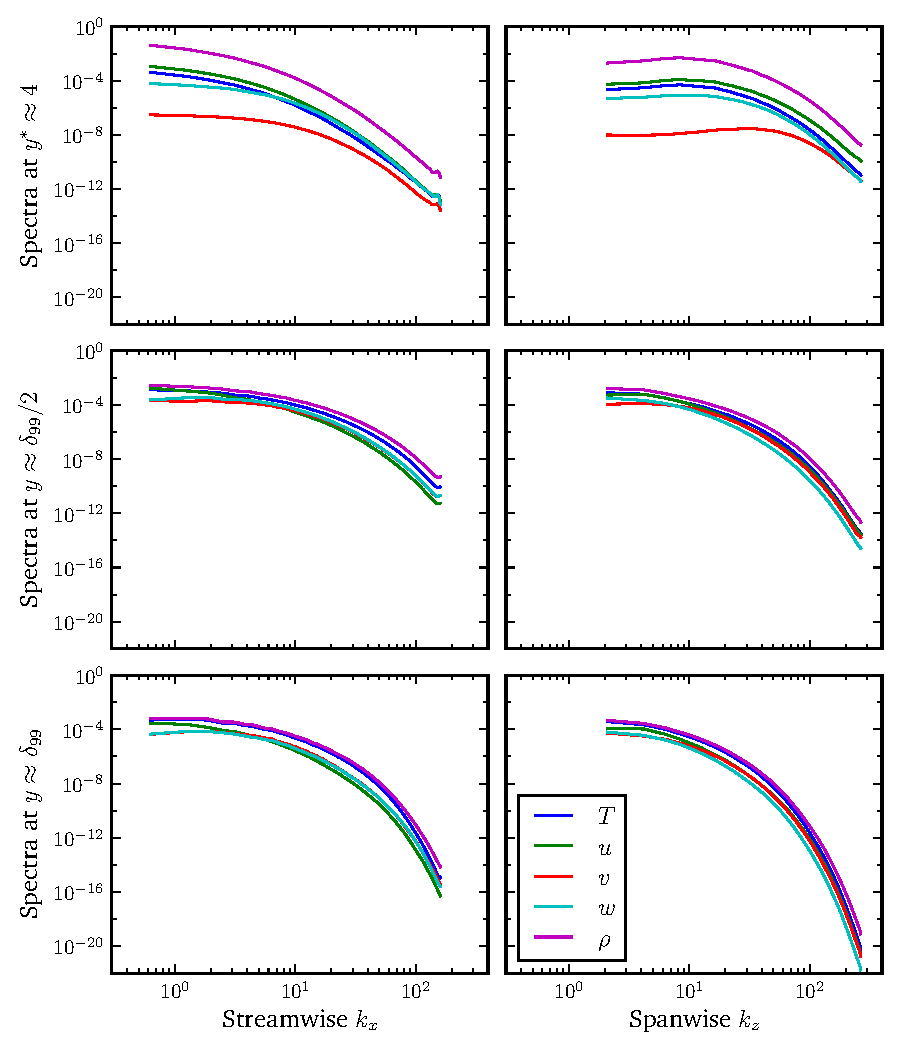
\includegraphics[width=\textwidth]{spectra-turb3199}
\caption{%
    One-dimensional, unnormalized Fourier energy spectra for case
    t3.199.\label{fig:spectra-t3199}
}
\end{figure}

% COMPARE ColemanJFM1995 Figure 1, Guarini JFM 2000 Figure 1
\begin{figure}
\centering
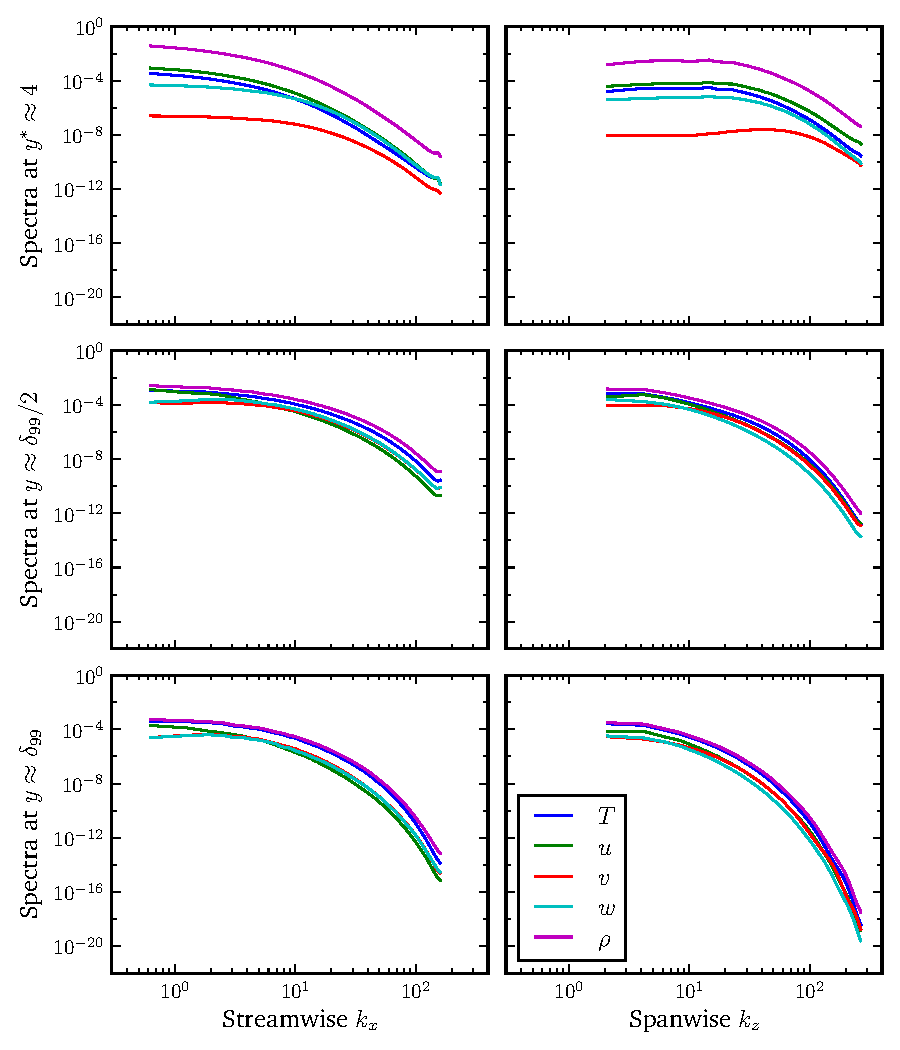
\includegraphics[width=\textwidth]{spectra-turb4134}
\caption{%
    One-dimensional, unnormalized Fourier energy spectra for case
    t4.134.\label{fig:spectra-t4134}
}
\end{figure}

% COMPARE ColemanJFM1995 Figures 3-4, Guarini JFM 2000 Figure 2
\begin{figure}
\centering
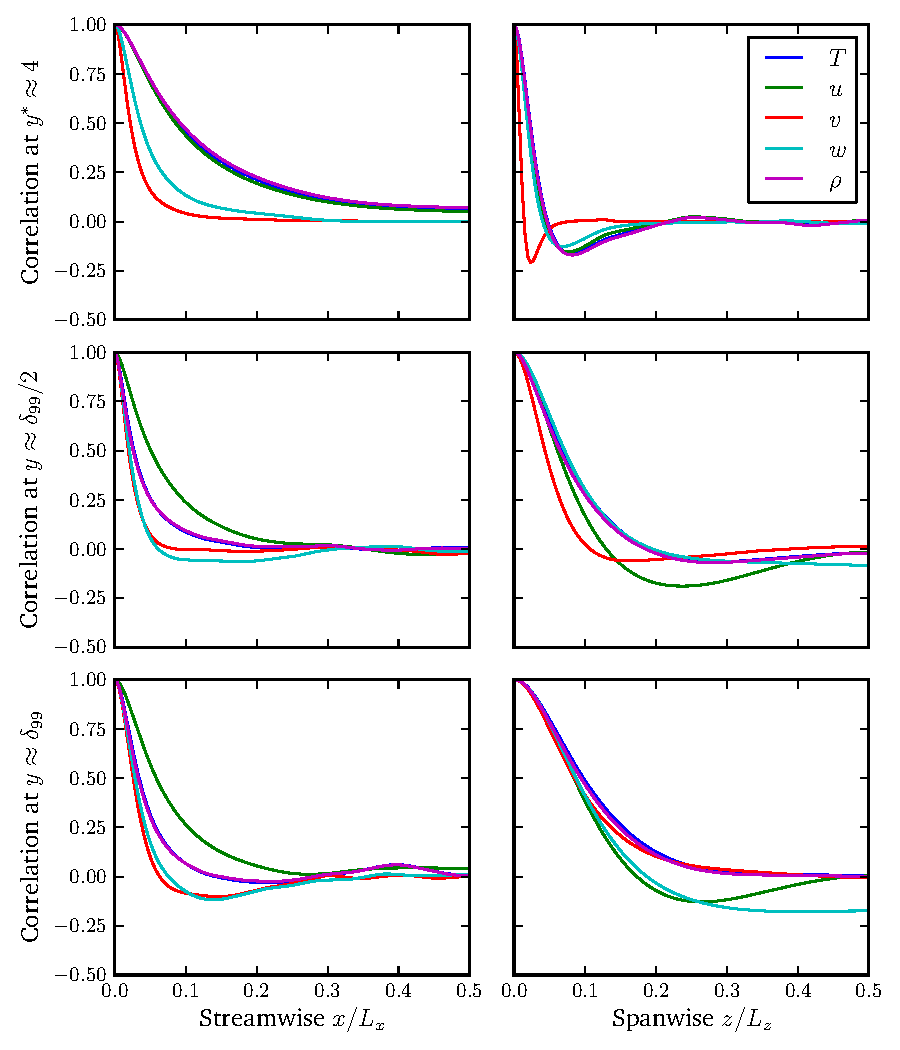
\includegraphics[width=\textwidth]{autocorr-turb3199}
\caption{%
    Two-point correlations for simulation t3.199.\label{fig:autocorr-t3199}
}
\end{figure}

% COMPARE ColemanJFM1995 Figures 3-4, Guarini JFM 2000 Figure 2
\begin{figure}
\centering
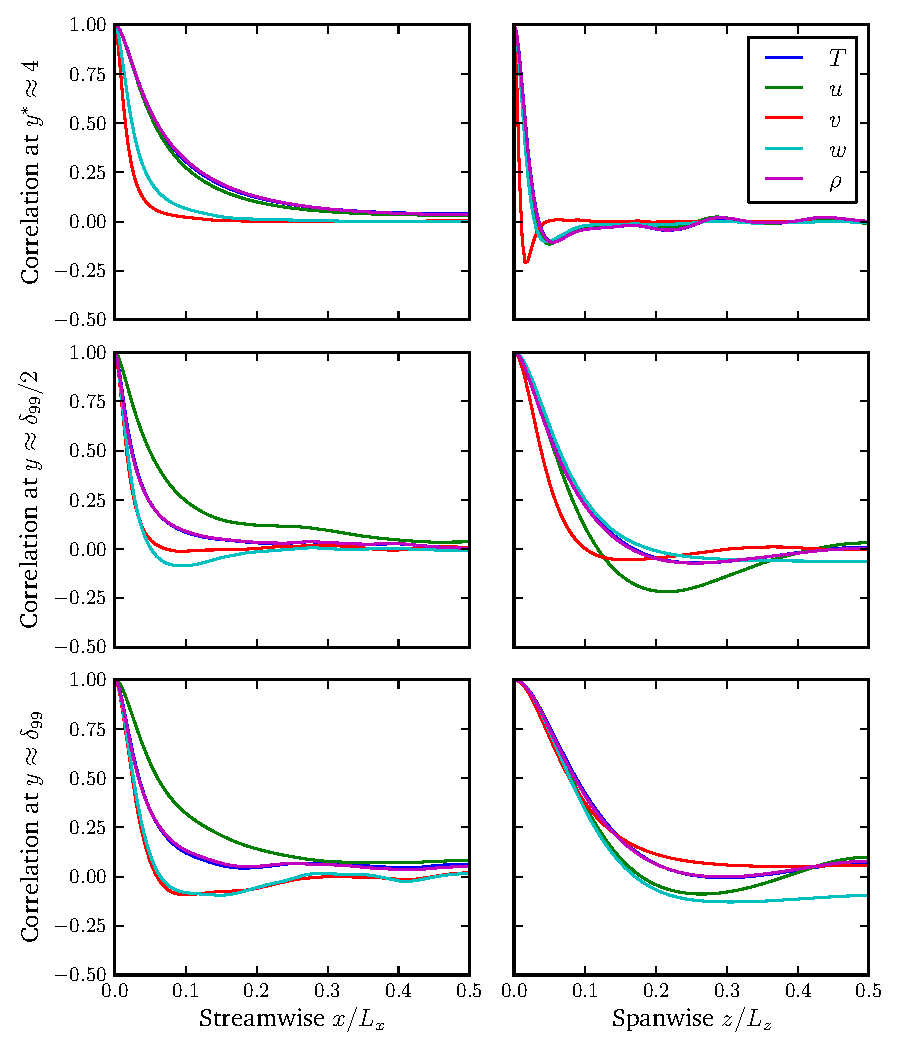
\includegraphics[width=\textwidth]{autocorr-turb4134}
\caption{%
    Two-point correlations for simulation t4.134.\label{fig:autocorr-t4134}
}
\end{figure}

The one-dimensional Fourier spectra, shown for primitive variables in
Figures~\ref{fig:spectra-t3199} and~\ref{fig:spectra-t4134}, indicate that the
present simulations are better resolved in the periodic directions than
those of \citeauthor{Coleman1995Numerical}.
%
The streamwise spectra at $y^{\ast}=y \sqrt{\tau_w / \rho} / \nu \approx{}4$ demonstrate that $L_x$ was
slightly smaller than required to eliminate artifacts from the periodic boundary
conditions.  This is corroborated by the two-point correlations in
Figures~\ref{fig:autocorr-t3199} and~\ref{fig:autocorr-t4134} which show $T$,
$u$, and $\rho$ not decorrelating fully at $x/L_x=0.5$.  However, the streamwise
correlations exhibit less coherence than those of
\citeauthor{Coleman1995Numerical} and \citeauthor{Guarini2000Direct} and, like
those authors, we anticipate finite domain effects to have little impact on the
results presented here.  Aside from the spanwise velocity~$w$, spanwise
coherence far from the wall is smaller than \citeauthor{Guarini2000Direct}
reported and is found acceptable.
%
The increase in $w$ correlation as $y$ increases, also observed by
Victor Topalian (personal communication), is thought to be a benign artifact of the
homogenization.
%
Given the quality of the spectra, evidently $L_z$ could have been larger without
incurring extra computational expense and without adversely decreasing spanwise
resolution.

In the wall-normal direction for case t3.199, collocation point
$y_{15}^{+}\approx{}10.4$, 178~points were inside $\delta_{99}$,
and $\left.\Delta{}y^{+}\right|_{y=\delta_{99}} \approx 10.7$.
For case t4.134, $y_{13}^{+}\approx{}10.1$, 180~points were inside
$\delta_{99}$, and $\left.\Delta{}y^{+}\right|_{y=\delta_{99}}
\approx 15.0$.  To account for the considerable density and
temperature gradients arising from holding wall temperatures
fixed, the wall-normal grid spacings are more appropriately
assessed when scaled by semi-local units~\citep{Huang1995Compressible,Morinishi2005Study}
%
which use either $u^\ast_\tau = \sqrt{\tau_w / \rho}$ or $\delta^\ast_\nu = \nu / u^\ast_\tau$.
%which are similar to
%$\delta_\nu$ and $u_\tau$ except that local density and viscosity are used in
%lieu of wall values.
For simulation t3.199, collocation point
$y_{27}^{*}\approx{}10.1$ and $\left.\Delta{}y^{*}\right|_{y=\delta_{99}}
\approx 1.6$.  For case t4.134, $y_{24}^{*}\approx{}10.3$ and
$\left.\Delta{}y^{*}\right|_{y=\delta_{99}} \approx 2.2$.

Both simulations used linear implicit time discretization only for
operators involving derivatives in the wall-normal direction and,
given the lessons learned in \autoref{sec:channel_runs} regarding the
aggressiveness of the eigenvalue estimates from \autoref{sec:wallnormaleigval},
time step safety factors of 0.35 were selected.  As measured by
time-to-solution, linear implicitness in three directions was equally but no
more performant than the wall-normal-only variant.  The latter was chosen as it
used smaller time steps and therefore was expected to better resolve flow
dynamics.  The column ``turnovers'' conveys the time over which the statistical
ensemble was collected divided by $\delta_{99}/u_\tau$.  The ensemble for cases
t3.199 and t4.134 includes 764 and 837 instantaneous planar averages over $x$
and $z$ which were collected \emph{in situ} from the simulations.  Uncertainties
were estimated from the temporal trace of these equispaced samples following
procedures outlined in \autoref{eq:uqaccounting}.

\autoref{tbl:table_turb_hbl_params} documents the fixed temporal slow growth
rates $\operatorname{gr}_{t_0}\!\left(\Delta\right)$, the isothermal wall
temperatures, and the wall blowing rates.  It shows that the homogenization held
$\delta_{99} \approx 1$ and that the desired $\Reynolds[99]$ and $\Mach[99]$
conditions were produced.  The remaining columns confirm that simulations t3.199
and t4.134 indeed correspond to their namesake locations in
Figures~\ref{fig:cevisslam_summary1} and~\ref{fig:cevisslam_summary_fpg} save
for possessing $\Reynolds[\theta]$ representative of those found in in
\autoref{tbl:BaumanCEVConditionsPerfect}.

\autoref{tbl:table_turb_hbl_fpg} characterizes the favorable pressure gradients
found in the two simulations in a variety of ways.  The desired
inviscid pressure gradient parameter $p_{e,\xi}^\ast$, defined in \eqref{eq:defnpexi},
is listed alongside the observed result at $\delta_{99}$ labeled
$p_{99,\xi}^{\ast}$.  The inviscid base flow design procedure from
Appendix~\ref{sec:radialflow} produced the target pressure gradient strength to
within 0.6\%.  Comparing the tabulated values against
\autoref{fig:cevisslam_summary_fpg}, the simulated values of Launder's
acceleration parameter $K$ are between the bands shown calculated from fully
laminar Orion MPCV computations.  Simulation t3.199 shows reasonable agreement
with the expected Pohlhausen parameter $K_s$ from the same figure while
simulation t4.134 is more than 50\% too large.  However, the $K_s$ values
computed from the MPCV source data are suspect as they possess appreciable numerical
artifacts.  Both simulations produced $\Lambda_n$ values roughly a factor of two
less than the MPCV data but the discrepancy is not surprising as the wall shear
$\tau_w$ entering into $\Lambda_n$ was not specified \emph{a priori}.
We consider the inviscid base design procedure to be successful because it
closely reproduced the desired condition on $p_{99,\xi}^\ast$ while yielding
pressure gradients not too dissimilar from the MPCV data when quantified using
other metrics.

\autoref{tbl:table_turb_hbl_edgewall} conveys several quantities of interest
from the simulations.  As expected, the prescribed wall temperatures $T_w/T_0$
produce larger densities and lower viscosities near the wall.
%
Despite its wall-normal velocity at the edge being positive, simulation t4.134
uses subsonic inflow boundary conditions because of how the homogenization
causes inputs $L_y$ and $\operatorname{gr}_{t_0}\!\left(\Delta\right)$ to modify
the wall-normal inviscid characteristics as discussed in
\autoref{sec:impacthomovisc}.
%
On account of wall injection, friction Reynolds
number $\Reynolds[\tau]{}$ is higher and skin friction $c_f$ is lower than
might be expected based upon $\Reynolds[\theta]{}$ and
$\Mach[99]{}$~\citep{Sumitani1995Direct, Smits2005Turbulent}.  To ease
comparing surface heating predictions against the present results, the
nondimensional heat flux $B_q$ and the Nusselt number $\textrm{Nu}_{99}$
%based on $T_{99}$ and $T_w$
are also tabulated.

%%%%%%%%%%%%%%%%%%%%%%%%%%%%%%%%%%%%%%%%%%%%%%%%%%%%%%%%%%%%%%%%%%%%%%%%%%%%%%
\section{A Note on Integral Thicknesses and the Clauser Parameter}
\label{sec:bldata_integrallengths}

The omissions of the displacement thickness $\delta^\ast$, the momentum
thickness $\theta$, and the Clauser parameter
$\beta$~\citep{Clauser1954Turbulent} from the above tables merit explanation.
That explanation requires revisiting the classical definitions of the two
thicknesses to properly account for the presence of the nonuniform inviscid
base flows which were used to enforce nonzero pressure gradients.  Along the
way, the two related integral thickness Reynolds numbers accommodating
nonuniform base flows will be derived.

As explained in, for example, \citet[\textsection{}9.2]{Dowling2012} the
displacement thickness $\delta^\ast$ is the distance by which the wall would
have to be displaced upward in a hypothetical frictionless flow to maintain the
same mass flux as that in the viscous flow.  That is, $\delta^\ast$ is the
length satisfying
\begin{align}
    \int_0^\infty {\rho u}_\text{viscid} (y) \, \mathrm{d}y
&=
    \int_{\delta^\ast}^\infty {\rho u}_\text{inviscid} (y) \, \mathrm{d}y.
\end{align}
Formally the upper limit may be replaced by any sufficiently large, finite
value because ${\rho u}_\text{viscid} \to {\rho u}_\text{inviscid}$ as
$y\to\infty$.  Assuming our domains are large enough,
\begin{align}
    \int_0^{L_y} {\rho u}_\text{viscid} (y) \, \mathrm{d}y
&=
    \int_{\delta^\ast}^{L_y} {\rho u}_\text{inviscid} (y) \, \mathrm{d}y.
    \label{eq:dispthick_general}
\end{align}
One can obtain a simplification often taken as a definition~\citep[Equation
10.95]{Schlichting2000Boundary},
\begin{align}
    \delta^\ast
&=
    \int_0^{L_y} 1 - \frac{{\rho u}_\text{viscid} (y)}{\rho_e u_e} \, \mathrm{d}y,
    \label{eq:dispthick_const}
\end{align}
for the special case of a uniform inviscid flow where ${\rho u}_\text{inviscid}
(y) = \rho_e u_e$.
%
Multiplying by $\rho_e u_e / \mu_e$, recognizing the displacement Reynolds
number $\Reynolds[\delta^\ast]{}$, and formally converting back to the
nonuniform inviscid base flow,
\begin{align}
    \Reynolds[\delta^\ast]{}
=
    \frac{\rho_e u_e \delta^\ast}{\mu_e}
&=
    \frac{\rho_e u_e}{\mu_e}
    \int_0^{L_y} 1 - \frac{{\rho u}_\text{viscid} (y)}{\rho_e u_e} \, \mathrm{d}y,
\notag\\&=
    \mu_e^{-1}
    \int_0^{L_y} \rho_e u_e - {\rho u}_\text{viscid} (y) \, \mathrm{d}y,
\notag\\&\approx
    \mu_e^{-1}
    \int_0^{L_y} {\rho u}_\text{inviscid}(y) - {\rho u}_\text{viscid} (y) \, \mathrm{d}y.
    \label{eq:dispreynolds_general}
\end{align}
A constant viscosity, here chosen to be $\mu_e$, should scale the
above integral when defining $\Reynolds[\delta^\ast]{}$.  There is no sensible
way to incorporate dimensions of inverse viscosity into its integrand's left
term thus permitting $\mu^{-1}(y)$ to multiply the right term.

\begin{figure}
\centering
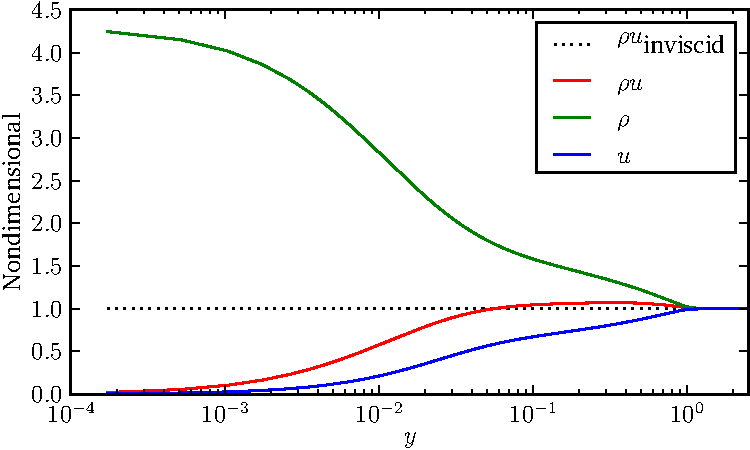
\includegraphics[]{delta1weird}
\caption{%
    The inviscid base flow and viscous flow profiles for simulation
    t4.134\label{fig:delta1weird}
}
\end{figure}

Mean profiles from simulation t4.134 pictured in \autoref{fig:delta1weird} are
the impetus for recalling the general displacement thickness
balance~\eqref{eq:dispthick_general} as well as its
simplification~\eqref{eq:dispthick_const}.  Progressing from the cold wall at
$y=0$ to the boundary layer edge at $y=\delta_{99}\approx{}1$, the streamwise
velocity increases, the density drops considerably, and the momentum in the
viscous flow exceeds that of the inviscid base flow.
%
Evaluating integral~\eqref{eq:dispthick_const} taking $\rho_e u_e$ from
$\delta_{99}$ produces $\delta^\ast/l_0 = -0.03923$.
%
Interpreting this negative $\delta^\ast$ through the usual displacement effect
intuition, for simulation t4.134 introducing the cold plate into the inviscid
profile increases the mass flow rate because it significantly increases the
near-wall density.
%
Negative $\delta^\ast$ are reported for exotic flows but
seem uncommon~\citep[e.g.][]{Fergason2001Simulations, Brown1952Solutions}.
%
The flow, however, need not be exotic.  The zero-pressure-gradient boundary
layer forming on a sufficiently cold, flat plate in laminar air will exhibit a
negative displacement thickness (Truman E. Ellis, personal communication).
%
Evaluating the right hand integrand for the more correct
balance~\eqref{eq:dispthick_general} behaves unusually--- the shape of the inviscid base flow when $y < 0$ does not
influence the viscous solution on $y\in\left[0,L_y\right]$ but it
impacts $\delta^\ast$.
%
%%% To elaborate, in the ``subsurface'' region where $y<0$ any
%%% ${\rho u}_\textrm{inviscid} (y)$ from a stationary solution
%%% of the inviscid Euler equations is admissible provided that
%%% the solution agrees with the chosen base flow at finitely many
%%% collocation points $y_l\in\left[0,L_y\right]$.  This ability to
%%% freely choose the subsurface inviscid profile and thereby, on a
%%% fixed computational grid, adjust $\delta^\ast$ without consequences
%%% perhaps surprisingly makes $\delta^{\ast} < 0$ somewhat ill-defined
%%% per~\eqref{eq:dispthick_general}.
%
For this reason, a generalization of~\eqref{eq:dispthick_const},
\begin{align}
    \delta^\ast
&=
    \int_0^{L_y} 1 - \frac{{\rho u}_\text{viscid} (y)}
                          {{\rho u}_\text{inviscid} (y)} \, \mathrm{d}y,
    \label{eq:dispthick_final}
\end{align}
is selected as a definition and evaluating it shows
$\delta^\ast = -0.03918$ in simulation t4.134.
%
Therefore, $\Reynolds[\delta^\ast]$ must be negative and indeed
evaluating~\eqref{eq:dispreynolds_general} finds $\Reynolds[\delta^\ast] =
-129$.
%
The Clauser parameter $\beta=\frac{\delta^\ast}{\tau_w} \frac{\partial
p}{\partial x}=0.1608$ is positive in this favorable pressure gradient flow,
contrary to expectations~\citep[e.g.][]{Bowersox1996Turbulence}, because of
negative displacement effects.
%
Simulation t3.199 also exhibits the actual momentum exceeding the inviscid
profile momentum (not shown) but possesses $\delta^\ast/l_0=0.006429$,
$\Reynolds[\delta^\ast]=15.8$, and $\beta=-0.02148$;  $\beta$
in no way communicates the strength of the pressure gradient as many
authors term 0.1 a strong magnitude~\citep{Smith1994Effects,Luker2000Influence}.

Negative displacement effects are not evident in the reacting, fully
turbulent Orion MPCV data from~\autoref{tbl:BaumanCEVConditions}
($\delta^\ast/\delta\approx 0.113$) nor do they appear in the fully
laminar results depicted in \autoref{fig:cevisslam_summary_fpg} ($\beta<0$
leeward of the stagnation point).  These effects might not occur because
of the higher edge Prandtl numbers in those reacting simulations (see
$\Prandtl[e]$ in \autoref{fig:cevisslam_summary1}) because as the Prandtl number
increases it causes the thermal boundary layer to grow more slowly relative to
the momentum boundary layer.

The momentum thickness $\theta$ quantifies the momentum defect relative to the
inviscid flow after removing displacement effects.  That is, $\theta$ is the
length satisfying
\begin{align}
    \int_0^{L_y} {\rho u^2}_\text{viscid} (y) \, \mathrm{d}y
&=
    \int_{\theta}^{L_y}  {\rho u^2}_\text{inviscid} (y) \, \mathrm{d}y
  - \int_0^{\delta^\ast} {\rho u^2}_\text{inviscid} (y) \, \mathrm{d}y
    \label{eq:momthick_general}
\end{align}
given fixed $\delta^\ast$ where again the upper limit has been truncated to
the domain extent.
%
The commonly seen degenerate form of the above balance, often taken as a
definition when ${\rho u}_\text{inviscid} (y) = \rho_e u_e$, is recovered as
follows:\footnote{%
    \citet[page 214]{Smits2005Turbulent} and \citet[page
    324]{LiepmannRoshko2002} present result~\eqref{eq:momthick_incomp}.
    \citet[Equation 10.95]{Schlichting2000Boundary} made an
    error in their definition for $\theta$.
}
\begin{align}
    \int_0^{L_y} {\rho u^2}_\text{viscid} (y) \, \mathrm{d}y
&=
    \rho_e u_e^2 \left(L_y - \theta\right)
  - \rho_e u_e^2 \delta^\ast
\notag\\
    \rho_e u_e^2 \theta
&=
    \rho_e u_e^2 L_y
  - \int_0^{L_y} {\rho u^2}_\text{viscid} (y) \, \mathrm{d}y
  - u_e \left[\rho_e u_e \delta^\ast\right]
\notag\\
&=
    \int_0^{L_y} \rho_e u_e^2 - {\rho u^2}_\text{viscid} (y) \, \mathrm{d}y
  - u_e \left[
        \int_0^{L_y} \rho_e u_e - {\rho u}_\text{viscid} (y) \, \mathrm{d}y
    \right]
\notag\\
    \theta
&=
    \int_0^{L_y}
        \left(1 - \frac{{\rho u^2}_\text{viscid} (y)}{\rho_e u_e^2}
    \right)  \, \mathrm{d}y
  - \int_0^{L_y}
        \left(1 - \frac{{\rho u}_\text{viscid} (y)}{\rho_e u_e}
    \right)  \, \mathrm{d}y
\notag\\
&=
    \int_0^{L_y} \frac{{\rho u}_\text{viscid} (y)}{\rho_e u_e} \left(
        1 - \frac{{u}_\text{viscid} (y)}{u_e}
    \right)  \, \mathrm{d}y
    \label{eq:momthick_incomp}.
\end{align}
Unlike the analogous~\eqref{eq:dispthick_const}, only nonnegative values
are possible.
%
%\citet[\textsection{}9.2]{Dowling2012} provides the interpretation that, in
%this special case, $\rho_e u_e^2 \theta$ is nothing but the momentum loss in
%the viscous flow because of the presence of the boundary layer.
%
Multiplying by $\rho_e u_e/\mu_e$ and formally converting back to the nonuniform
base flow,
\begin{align}
    \Reynolds[\theta]{}
=   \frac{\rho_e u_e \theta}{\mu_e}
&=  \frac{\rho_e u_e       }{\mu_e}
    \int_0^{L_y} \frac{{\rho u}_\text{viscid} (y)}{\rho_e u_e} \left(
        1 - \frac{{u}_\text{viscid} (y)}{u_e}
    \right)  \, \mathrm{d}y
\notag\\
&=  \mu_e^{-1}
    \int_0^{L_y} {\rho u}_\text{viscid} (y) \left(
        1 - \frac{{u}_\text{viscid} (y)}{u_e}
    \right)  \, \mathrm{d}y
\notag\\
&\approx  \mu_e^{-1}
    \int_0^{L_y} {\rho u}_\text{viscid} (y) \left(
        1 - \frac{{u}_\text{viscid} (y)}{u_\text{inviscid} (y)}
    \right)  \, \mathrm{d}y.
    \label{eq:momreynolds_general}
\end{align}
Here, $\mu(y)$ could have been incorporated into the integrand, but it
was not for consistency with~\eqref{eq:dispreynolds_general}.

Defining $\theta$ via the general balance~\eqref{eq:momthick_general} is
problematic when negative displacement effects are present because, for
consistency, that approach should use $\delta^\ast$ from~\eqref{eq:dispthick_general}.
%
For this reason, generalizing~\eqref{eq:momthick_incomp} the present work uses
\begin{align}
    \theta
&=
    \int_0^{L_y} \frac{{\rho u}_\text{viscid} (y)}
                      {{\rho u}_\text{inviscid}(y)} \left(
        1 - \frac{{u}_\text{viscid} (y)}{u_\text{inviscid}(y)}
    \right)  \, \mathrm{d}y
\end{align}
and finds $\theta=0.1557$ and $\theta=0.1611$ for simulations t3.199 and t4.134,
respectively.  The generalization makes little difference--- assuming the base
flow was constant and directly evaluating~\eqref{eq:momthick_incomp} from
inviscid values at $y=\delta_{99}$ changes only the final reported digit in each
result.
%
Computed either way, the two spatiotemporal simulations have momentum
thicknesses larger than the reacting, fully turbulent Orion MPCV data
from~\autoref{tbl:BaumanCEVConditions} ($\theta/\delta\approx 0.134$).
%
The present simulation shape factors $H=\delta^\ast/\theta$ of $0.04129$ and
$-0.2432$ are well below standard turbulent boundary layer values and contrast
strongly with the fully turbulent MPCV result of $H\approx0.847$ acquired with
the aid of a Baldwin--Lomax model.
%
Momentum Reynolds numbers computed according
to~\eqref{eq:momreynolds_general} appeared in
\autoref{tbl:table_turb_hbl_params}.


%%%%%%%%%%%%%%%%%%%%%%%%%%%%%%%%%%%%%%%%%%%%%%%%%%%%%%%%%%%%%%%%%%%%%%%%%%%%%%


% Wall injection tends to activate near-wall turbulence, shear stress, heat fluxes \citet{Sumitani1995Direct}
% Injection stimulates the occurrence of quasicoherent streamwise vorticle structures which are associated with primary turbulence mechanisms \citet{Sumitani1995Direct}

%Turbulent Mach Number

\section{Turbulence Statistics}
\label{sec:bldata_stats}

This section reviews a collection of turbulent statistics for the present
simulations.  Comparisons to other work are included but are limited
because, as evidenced by their shape factors, these two cold-wall
spatiotemporally homogenized flows differ considerably from canonical boundary
layers.


\begin{figure}
\centering
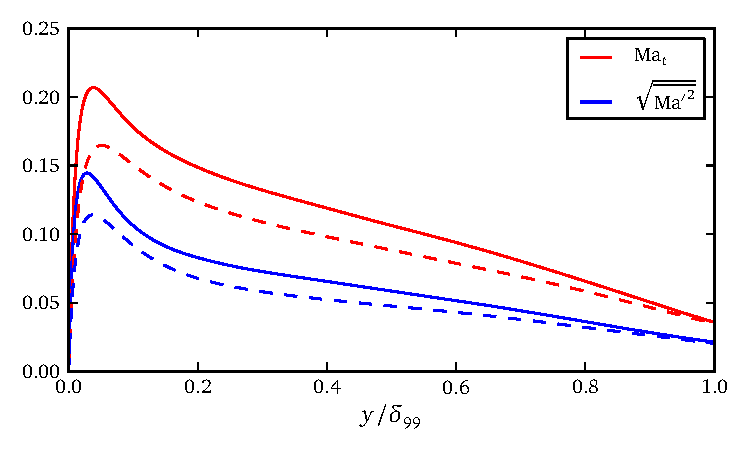
\includegraphics[]{hqd_mach}
\caption[Fluctuating Mach number profiles for simulations t3.199 and t4.134]{%
    Turbulent Mach number $\Mach[t]=\sqrt{2 k}/\bar{a}$
    and root-mean-squared local Mach number for simulations
    t3.199 (dashed) and t4.134 (solid).\label{fig:hdq_mach}
}
\end{figure}

\autoref{fig:hdq_mach} reports the turbulent Mach number $\Mach[t]{}$ and
root-mean-squared Mach number fluctuations.  Turbulence in both simulations
should only be weakly affected by compressibility effects because $\Mach[t]$ is
well below 0.3~\citep{Smits2005Turbulent}.  Local shocklets are not expected and
so the smoothness assumptions inherent to the numerical approach
from~\autoref{sec:techniques} are valid.  Consistent with
\citet{Guarini2000Direct}, the peak $\Mach[t]$ is slightly offset from the
root-mean-square profile because the former includes contributions from all
three velocity components while the latter uses only streamwise information.  On
this plot, and on the remainder of the plots in this section using abscissa
$y/\delta_{99}$, simulation t4.134 shows sharper near-wall gradients because its
$\Reynolds[\theta]$ is larger than simulation t3.199.  Peak magnitudes for
simulation t4.134 match a $\Mach[e]=1.2$ and $\Reynolds[\theta]{}=420$ simulation by
\citet{Topalian2014Temporal} employing temporal
homogenization~\eqref{eq:temporalhomogenization} and also targeting Orion MPCV
cold, blowing wall conditions.  The introduction of spatial homogenization terms
within the model seems to have no impact on these curves.

\begin{figure}[p]
\centering
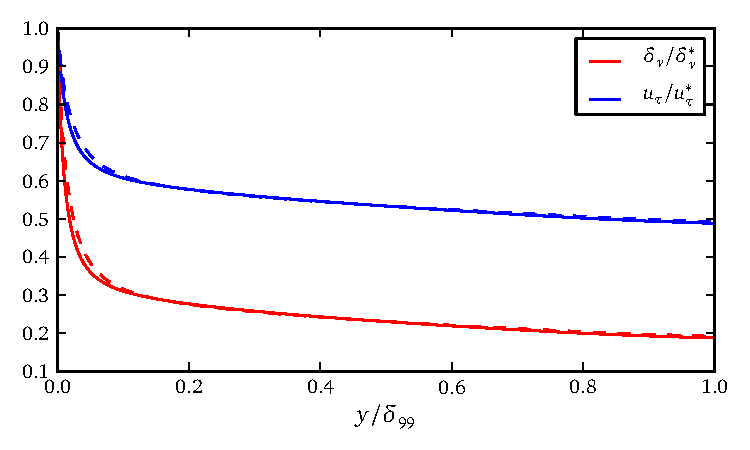
\includegraphics[]{hqd_star}
\caption[Wall versus semi-local scaling for simulations t3.199 and t4.134]{%
    Comparison of viscous length and velocity scales using wall and
    semi-local units~\citep{Huang1995Compressible} in simulations t3.199
    (dashed) and t4.134 (solid).\label{fig:hdq_star}
}
\end{figure}

\begin{figure}
\centering
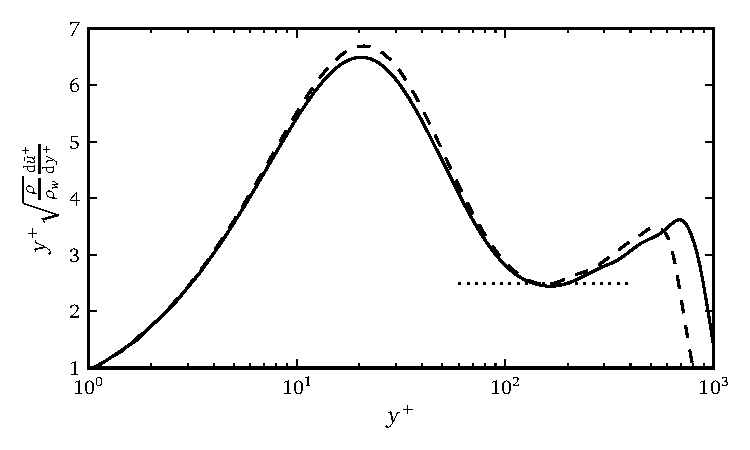
\includegraphics[]{hqd_inner}
\caption[Examination of inner scaling in simulations t3.199 and t4.134]{%
    Examination of inner scaling in simulations t3.199
    (dashed) and t4.134 (solid).
    For
    reference, the horizontal line shows $1/\kappa$ for
    $\kappa=0.40$.\label{fig:hdq_inner}
}
\end{figure}

Though compressibility is weak, \autoref{fig:hdq_star} shows that for these
large $T_{99}/T_w$ ratios variable density effects are strongest near the wall and
they continue throughout the boundary layer.  This is consistent with
$\Prandtl{}=0.7<1$ and the earlier discussion of very small or negative
displacement effects.  \autoref{fig:hdq_inner} shows an inner scaling plot
appropriate for compressible boundary layers~\citep{Chassaing2010Variable}.  In
a logarithmic inner region, one anticipates $\sqrt{\frac{\bar{\rho}}{\rho_w}}
\frac{\partial{\bar{u}^{+}}}{\partial y^{+}} = \frac{1}{\kappa y^{+}}$ which
does not appear because of the modest $\Reynolds[\theta]{}$ in these
simulations.  A von K\'arm\'an constant $\kappa$ of 0.40 predicts the tangent
where a logarithmic region would be expected at higher $\Reynolds[\theta]{}$.
In accordance with these two plots, semi-local units primarily will be used in
the remainder of the chapter.

Figures~\ref{fig:profile-t3199} and~\ref{fig:profile-t4134} show
nondimensional mean profiles and Reynolds stresses with the latter in semi-local
units.  The horizontal axes in the upper and lower images in the figures align
so that one can visually translate from $y^\ast$ to $y/\delta_{99}$.  Based on
techniques from \autoref{eq:uqaccounting}, uncertainties in the mean profiles
are presented in the upper right of each figure.  Qualitatively the uncertainty
profiles are similar between the two simulations though t3.199 shows somewhat
higher near-wall and mid-layer values and downward trends are more pronounced as
$y/\delta_{99}\to{}1$ in t4.134.  The peak uncertainties are modestly higher in
the higher $\Reynolds[\theta]$ case.  Importantly, the time step safety factor used
in these simulations did not produce the near-wall jaggedness that was visible
in~\autoref{fig:basic3k15} and so the temporal resolution is not suspect.
Turning to the lower half of the figure, the lower $\Mach[99]{}$ t3.199 shows a
slightly larger maximum $\widetilde{{u^{\prime\prime}}^2}$.  Maximum values are
higher than those found by \citet[Figure 6]{Guarini2000Direct} and
\citet[Figure 18]{Coleman1995Numerical} which is consistent with wall
blowing~\citep{Sumitani1995Direct}.  Uncertainties in the fluctuating quantities
grow as the edge of the boundary layer is approached but that is attributed to
the normalization by the small mean value found there.

Similar uncertainty estimates for over 225 Reynolds averaged scalar quantities
and their wall-normal derivatives were generated from \emph{in situ}
instantaneous averages taken over the streamwise and spanwise directions.  They
are not presented in this document but are available for calibration or modeling
purposes per Appendix~\ref{sec:archiving}.

\begin{figure}
\centering
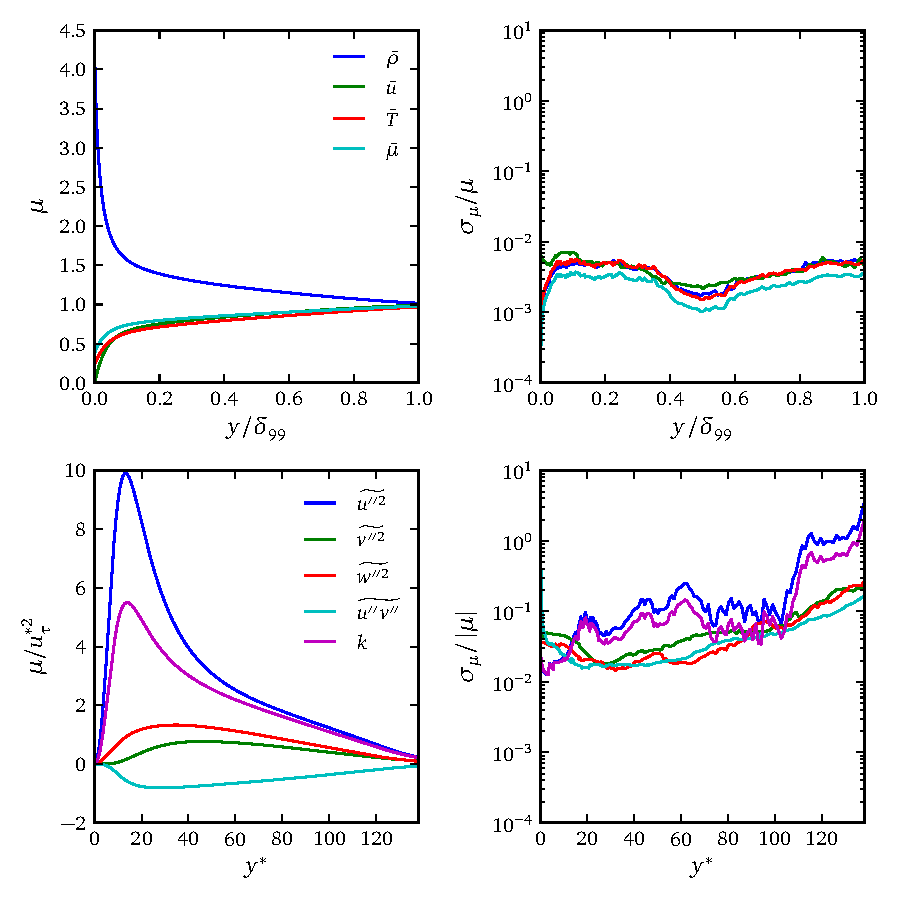
\includegraphics[width=\textwidth]{profile-t3199}
\caption[Profiles with quantified uncertainty for simulation t3.199]{%
    Reynolds-averaged primitive profiles (upper left) and Favre-averaged
    Reynolds stresses (lower left) with estimated standard errors
    as a fraction of mean (upper right, lower right) for simulation
    t3.199.\label{fig:profile-t3199}
}
\end{figure}

\begin{figure}
\centering
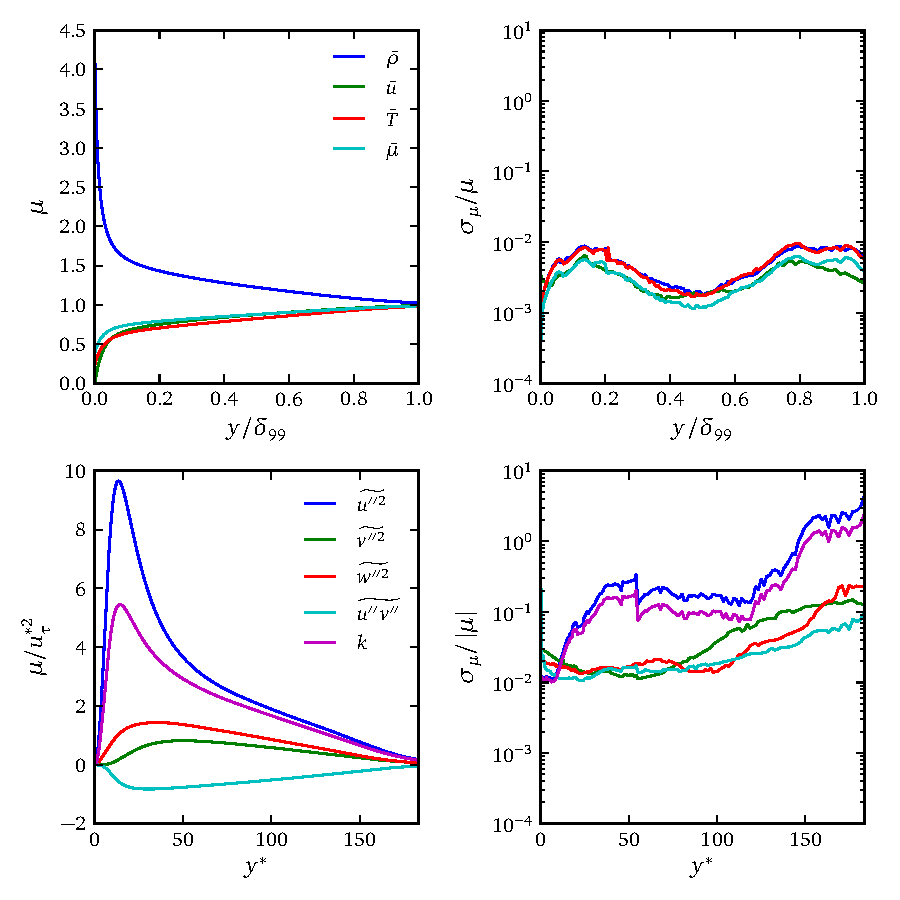
\includegraphics[width=\textwidth]{profile-t4134}
\caption[Profiles with quantified uncertainty for simulation t4.134]{%
    Reynolds-averaged primitive profiles (upper left) and Favre-averaged
    Reynolds stresses (lower left) with estimated standard errors
    as a fraction of mean (upper right, lower right) for simulation
    t4.134.\label{fig:profile-t4134}
}
\end{figure}

\begin{figure}[p]
\centering
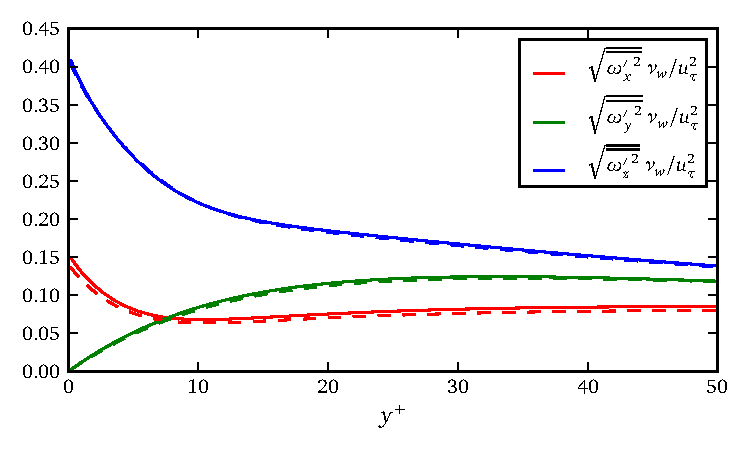
\includegraphics[]{hqd_vort}
\caption[RMS vorticity fluctuations for simulations t3.199 and t4.134]{%
    Root-mean-squared vorticity fluctuations normalized in wall units for
    simulations t3.199 (dashed) and t4.134 (solid).\label{fig:hdq_vort}
}
\bigskip\medskip
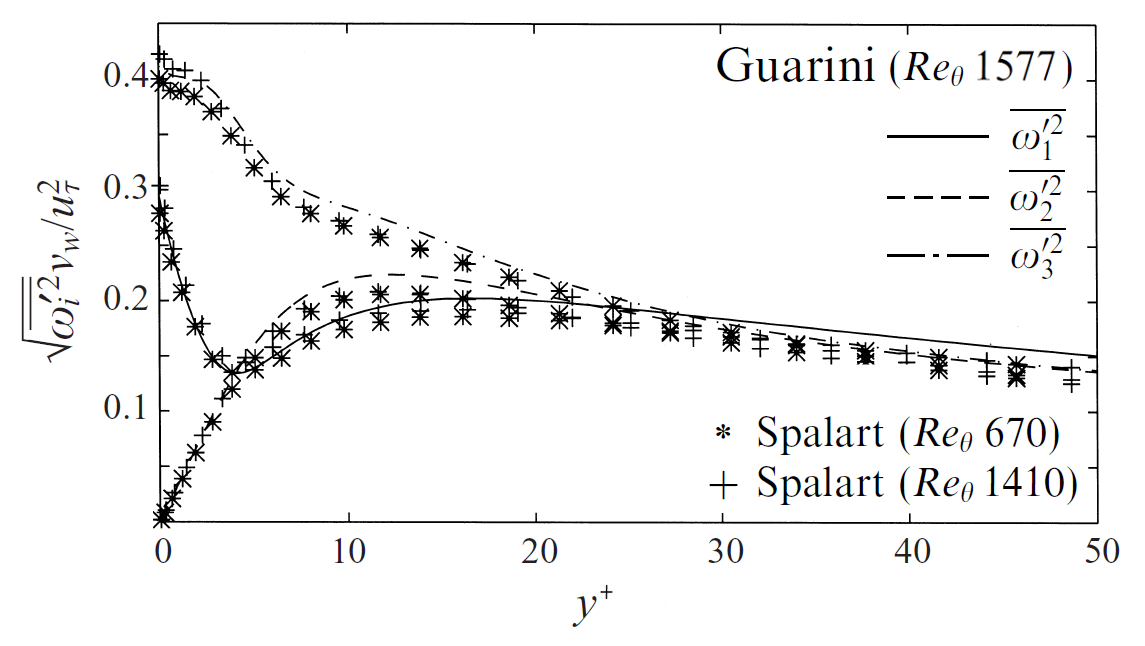
\includegraphics[width=5.2in]{GuariniJFM2000Figure8_Reworked}\hspace{1.5em}
\caption[RMS vorticity fluctuations reproduced from \citeauthor{Guarini2000Direct}]{%
    Root-mean-squared vorticity fluctuations from a $\Mach = 2.5$,
    adiabatic-wall spatially homogenized boundary layer by
    \citeauthor{Guarini2000Direct} and incompressible results by
    \citet{Spalart1988Direct}.  Reproduced from
    \citet{Guarini2000Direct}.\label{fig:hdq_vort_repo}
}
\end{figure}

\begin{figure}
\centering
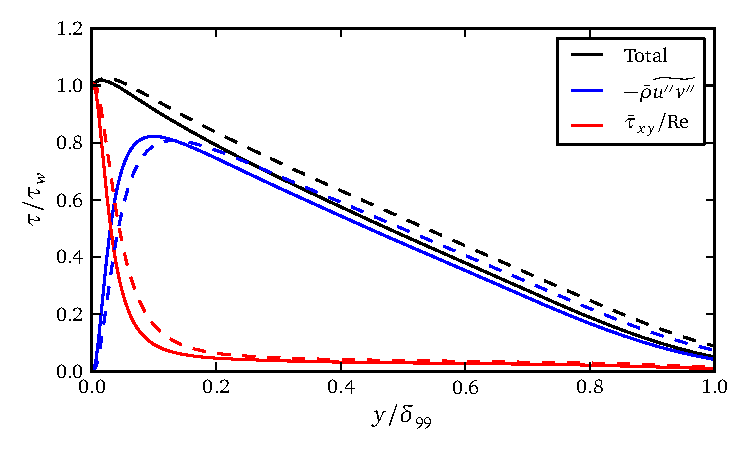
\includegraphics[]{hqd_tauxy}
\caption[Total shear stress contributions in simulations t3.199 and t4.134]{%
    Total shear stress contributions normalized in wall units for
    simulations t3.199 (dashed) and t4.134 (solid).\label{fig:hdq_tauxy}
}
\end{figure}

\autoref{fig:hdq_vort} displays root-mean-square vorticity fluctuations near the
wall normalized in wall units following \citet{Guarini2000Direct}.  Semi-local
units also caused the curves
to collapse for $y^{+}\lessapprox{}15$
in simulations t3.199 and t4.134
but they were less effective far from the wall (not shown).
Neither scaling removed the offset between the two simulations appearing in the
streamwise vorticity.  The spanwise maximum at the wall matches that shown in
\citet{Guarini2000Direct}, reproduced in \autoref{fig:hdq_vort_repo}.
The streamwise wall value is half what they
reported.  Qualitatively, the shapes have fewer curvature changes for
$y^{+}<20$, the near-wall local minimum in the streamwise data is more shallow,
and no localized peak appears in the wall-normal fluctuations.
These changes suggest the present simulations have atypical streamwise
vortex structures, perhaps as a consequence of wall blowing but the
spatiotemporal homogenization may also play a role.

\autoref{fig:hdq_tauxy} contains the total stress contributions for the streamwise
momentum equation.  The near-wall maxima are due to wall
injection~\citep{Sumitani1995Direct} with simulation t3.199 being slightly
higher because of its 18\% larger $v_w^{+}$.  \citet{Topalian2014Temporal},
using temporal homogenization~\eqref{eq:temporalhomogenization} in a
zero-pressure-gradient simulation at $\Mach[e]{}=1.2$ and
$\Reynolds[\theta]{}=420$, observed a blowing-related total stress maximum of
roughly 1.2 for a $v_w^{+}$ roughly
2.6x that used in simulation t4.134.  In contrast, t4.134 has maximum 1.0175.
The reduced maxima, relative to what might be expected if one scaled using only the blowing velocity,
are believed to be a consequence of the pressure gradient.

\begin{figure}
\centering
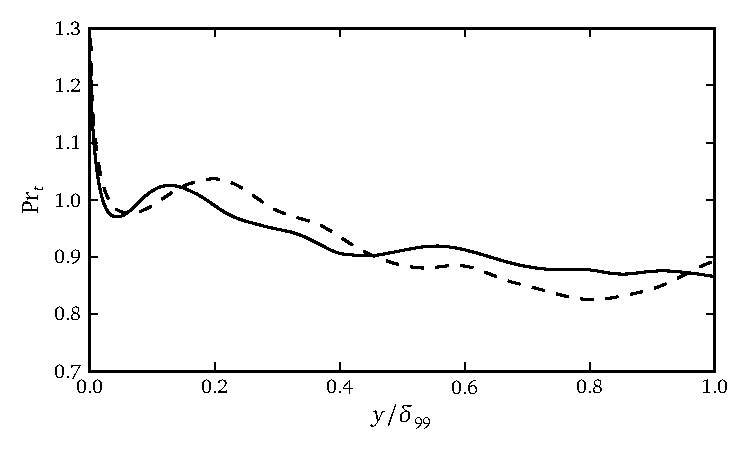
\includegraphics[]{hqd_prt}
\caption[Turbulent Prandtl number in simulations t3.199 and t4.134]{%
    Turbulent Prandtl number $\Prandtl[t]{} =
    \frac{\widetilde{u^{\prime\prime}v^{\prime\prime}}\partial_y\tilde{T}}
         {\widetilde{T^{\prime\prime}v^{\prime\prime}}\partial_y\tilde{u}}$
    for simulations t3.199 (dashed) and t4.134 (solid).\label{fig:hdq_prt}
}
\end{figure}

\autoref{fig:hdq_prt} reports the turbulent Prandtl number $\Prandtl[t]{}$ The
data shows perhaps unsettling waviness but similar fluctuations were observed
by \citet[Figure 14]{Guarini2000Direct}.  However, away from the wall the
present $\Prandtl[t]{}>0.8$ differs from their 0.7 result.

\begin{figure}[p]
\centering
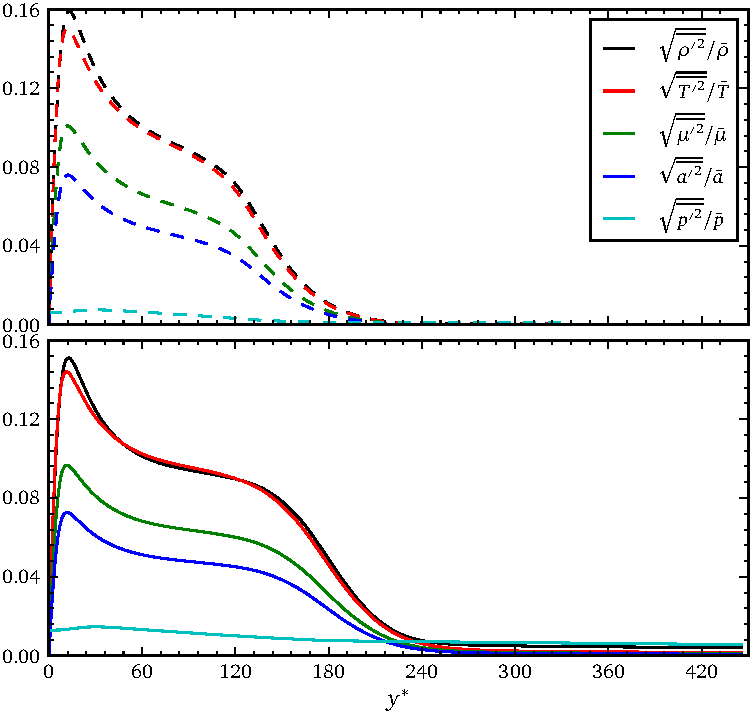
\includegraphics[]{hqd_fprop}
\caption[RMS thermodynamic fluctuations in simulations t3.199 and t4.134]{%
    Root-mean-squared thermodynamic property fluctuations normalized by local
    means for simulations t3.199 (above, dashed) and t4.134 (below,
    solid).\label{fig:hdq_fprop}
}
%\end{figure}
%\begin{figure}
%\centering
\bigskip\medskip
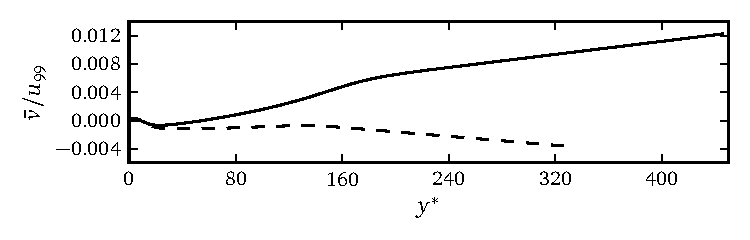
\includegraphics[]{hqd_v}
\caption[Mean wall-normal velocity for simulations t3.199 and t4.134]{%
    Mean wall-normal velocity normalized by the streamwise edge velocity
    for simulations t3.199 (dashed) and t4.134 (solid).\label{fig:hdq_v}
}
\end{figure}

\autoref{fig:hdq_fprop} contrasts root-mean-squared thermodynamic property
fluctuations between the two simulations.  Simulation t3.199 unexpectedly has
larger maxima than 4.134 for all quantities save pressure.
%
Most striking about these fluctuation magnitudes is that, unlike t3.199, in
t4.134 the pressure and density curves do not decay as fully outside
the boundary layer.
%
A fundamental difference between the inviscid base flow designs is one cause for
this behavioral change.  Simulation t3.199 is subsonic and therefore a favorable
pressure gradient is achieved, per Appendix~\ref{sec:radialflow}, with a
converging radial nozzle.  Supersonic simulation t4.134 uses a diverging radial
nozzle.

The mean wall-normal velocity $\bar{v}$ for these cases is shown in
\autoref{fig:hdq_v}.  The positive $\bar{v}$ at the wall quickly turns negative
in both simulations.  For t3.199 it stays negative thereafter causing
$\overline{\rho{}v}$ to become negative by $y/\delta_{99}\approx{}0.9$ (not
shown).  In t4.134, $\bar{v}$ changes sign before $y^\ast=80$ and proceeds to
increase throughout the upper portions of the domain with an appreciable curvature
change at the edge of the boundary layer.  At $y=L_y$ the wall-normal velocity
is more than 1\% of $u_{99}$ and $\overline{\rho v}$ is everywhere positive (not
shown).

A second potential cause for this lack of decay is the spatiotemporal
homogenization, possibly in conjunction with the numerical isothermal wall
and/or nonreflecting freestream boundary treatments.
%
It was noticed and subsequently confirmed by Topalian that, unlike
the temporal homogenization~\eqref{eq:temporalhomogenization}, the
spatiotemporal homogenization causes small point-to-point oscillations to appear
in the second derivative of pressure near both the lower and upper boundaries
(not shown).
%
This behavior can be reproduced by time-stepping a stationary one-dimensional
laminar solution even in zero-pressure-gradient cases for which the inviscid
base flow terms are inactive.
%
Transferring such a solution to progressively finer grids will cause the
pressure oscillations to eventually pollute other quantities and the numerical
solution to diverge.
%
Notably, only supersonic problems seem to be so affected.  Setting the modeled
defect growth rates (see \autoref{sec:imposing_fpg}) to be zero delays but does
not prevent the divergence.  The issue is not believed to be related to the
implicit treatment as time-stepping with fully explicit operators also shows
the same issue.
%
However, at wall-normal resolutions like that used for case t4.134 the precursor
pressure oscillations remain small and are not thought to spoil that
simulations' results.
%
Still, they suggest that, while suitable for calibration purposes and gross
behavioral investigations like those pursued in the next chapter, the
spatiotemporal homogenization and accompanying numerics in their current form
may not be appropriate for some studies of fundamental physics in supersonic
flows.

%%%%%%%%%%%%%%%%%%%%%%%%%%%%%%%%%%%%%%%%%%%%%%%%%%%%%%%%%%%%%%%%%%%%%%%%%%%%%%
\section{Favre-Averaged Equation Budgets}
\label{sec:bldata_budgets}

The spatiotemporal homogenization by \citet{Topalian2014Spatiotemporal} is
sufficiently new that term-by-term contributions to the averaged governing
equations, often called budgets, have not appeared in the literature.
%
This section presents such budgets, per the Favre-averaged Navier--Stokes
formulation documented in \autoref{sec:statevo}, to help quantify the impact of
this slow growth forcing on mean flow profiles.
%
Simulations t3.199 and t4.134 are particularly interesting for this purpose
because they fully exercise the novel inviscid base flow capabilities of the
homogenization.
%
In addition to characterizing the impact of the homogenization, this data
provides detailed information about the dynamics of complex boundary layers.

To begin, \autoref{fig:fans_rho} shows the budget for the Favre-averaged density~\eqref{eq:fans_mass}.  Though somewhat mundane, its presentation serves
three purposes.  First, it exhibits several choices made throughout the
remainder of this section.  Subsonic simulation t3.199 appears on the upper half
of the image with supersonic case t4.134 below.  Both halves use identical
ordinate ranges to communicate term-by-term budgets normalized by wall units.
Semi-local abscissa are chosen so that the two cases collapse permitting
comparisons of extrema locations between the upper and lower halves of the
figure.  The reader may find Figures~\ref{fig:profile-t3199}
and~\ref{fig:profile-t4134} helpful if converting locations from $y^\ast$ to
$y/\delta_{99}$ is desired.  A
logarithmic scale was selected so that near-wall, edge, and freestream behaviors of
the slow growth formulation can be assessed with one plot.  Second, \autoref{fig:fans_rho}
demonstrates several qualitative differences between the sub- and supersonic
behavior of the spatiotemporal formulation equipped with a favorable pressure
gradient inviscid base flow.  The subsonic case shows slow forcing, $\Ssd_\rho$,
changing sign inside the boundary layer while the supersonic forcing does not.
The boundary layer edge is quite apparent in the figure and $\Ssd_\rho$ changes
curvature dramatically in its vicinity.  Third, supporting comments in the last
section that the supersonic case is somewhat ill-behaved at the freestream
boundary, a kink appears only in the lower plot near $y=L_y$.

Figures~\ref{fig:fans_rho_u} and~\ref{fig:fans_rho_v} show budgets for
the two nontrivial scalar components of the Favre-averaged momentum~\eqref{eq:fans_mom}.  \autoref{fig:fans_rho_u}
demonstrates that $\Ssd_{\rho u}$ behaves similarly to $\Ssd_{\rho}$ with
regard to sub- versus supersonic conditions.  At $y^{\ast}\approx{}10$
simulation t4.134 shows a mildly more pronounced slow growth forcing peak and
again slight boundary condition artifacts at the freestream.  Slow growth makes
an appreciable contribution to the streamwise momentum balance
near the wall.  Turning to wall-normal momentum in
\autoref{fig:fans_rho_v}, the homogenization is not active and the subsonic and
supersonic cases are quite similar.

\autoref{fig:fans_rho_E} breaks apart the Favre-averaged total energy~\eqref{eq:fans_energy}.
Aside from anticipated Mach number-related
differences in viscous heating, the two simulations appear similar for
$y^\ast<40$.  Above that cutoff, slow growth and convection are much more active
in the supersonic case as a consequence of trends already shown in
\autoref{fig:hdq_v}.

Finally, the turbulent kinetic energy~\eqref{eq:fans_tke} appears for simulation
t3.199 in \autoref{fig:tke_t3199} and for t4.134 in \autoref{fig:tke_t4134}.
The upper half of each figure shows terms that strongly impact turbulent kinetic
energy $\rho k$.  The lower halves contain fine details that the upper plotting scale
would not permit visualizing.  The pressure dilatation and Reynolds heat
flux appear almost perfectly juxtaposed against one another because~\eqref{eq:lelecompresibility} was
used to eliminate the unclosed correlation $\overline{p'u''}$ from
formulation~\eqref{eq:fans_tke}.  The two terms are also summed in the lower
half.  As compared against a peak production of roughly 0.25 reported by
\citet{Schlatter2009Turbulent} for a spatially evolving zero-pressure-gradient
case at $\Reynolds[\theta]{}=670$, the present peak production is unexpectedly small
given that wall injection tends to energize
turbulence~\citep{Sumitani1995Direct}.
%
Importantly, Figures~\ref{fig:tke_t3199} and~\ref{fig:tke_t4134} demonstrate
that the \citet{Topalian2014Spatiotemporal} spatiotemporal homogenization
leaves the near-wall $\rho k$ budget largely unaffected.  The direct slow forcing
contribution $\overline{\Ssd_{\rho u}\cdot{}u^{\prime\prime}}$ is of the same
order of magnitude as the pressure terms for the present Mach numbers.

That last finding supports the expectation that a turbulence model calibrated to
accurately reproduce data from simulations t3.199 and t4.134 would be suitable
for use in predicting spatially evolving boundary layers with similar
characteristics.  Confirming this expectation by calibrating and validating
turbulence models is outside the scope of the current work.

\todo[inline]{%
    Fix weird figure size variability in the following figures---
    matplotlib padding is being finicky.
}

\begin{figure}
\centering
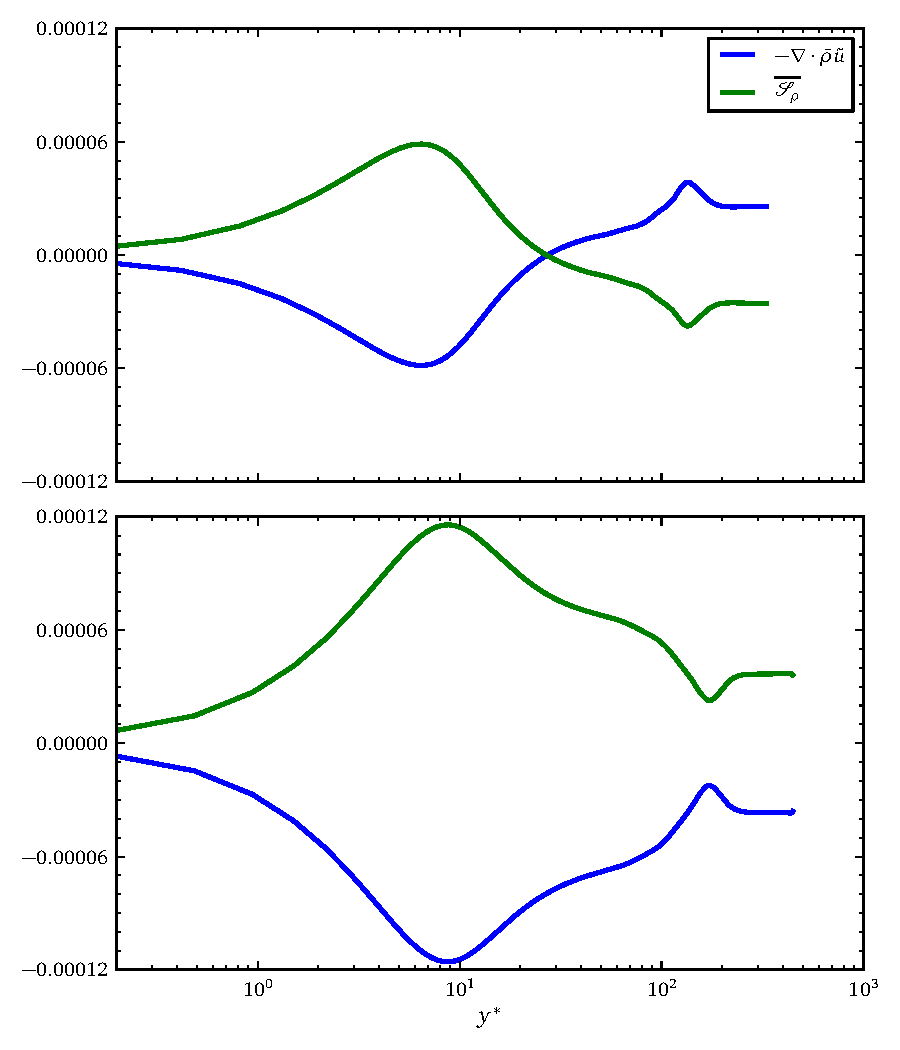
\includegraphics[width=\textwidth]{hqd_fans_rho}
\caption[Density equation budget for simulations t3.199 and t4.134]{%
    Budget for the Favre-averaged density~\eqref{eq:fans_mass}
    in simulations t3.199 (above) and t4.134 (below)
    normalized by $\rho_w u_\tau^2 / \nu_w$.\label{fig:fans_rho}
    % Normalize by \rho_w (\partial_y u)_w
}
\end{figure}

\begin{figure}
\centering
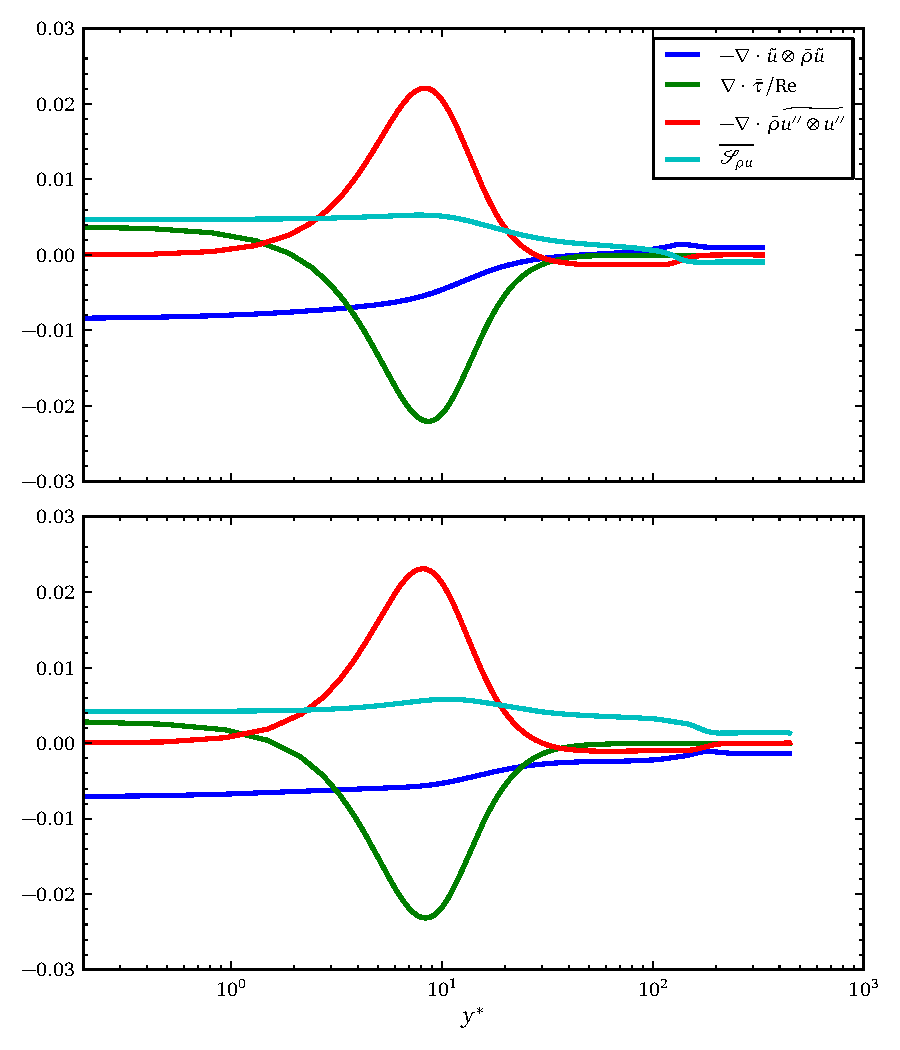
\includegraphics[width=\textwidth]{hqd_fans_rho_u}
\caption[Streamwise momentum equation budget for cases t3.199 and t4.134]{%
    Budget for the Favre-averaged streamwise momentum~\eqref{eq:fans_mom}
    in simulations t3.199 (above) and t4.134 (below)
    normalized by $\rho_w u_\tau^3 / \nu_w$.\label{fig:fans_rho_u}
    % Normalize by \rho_w (\partial_y u)_w u_\tau with u_tau having units u_0
}
\end{figure}

\begin{figure}
\centering
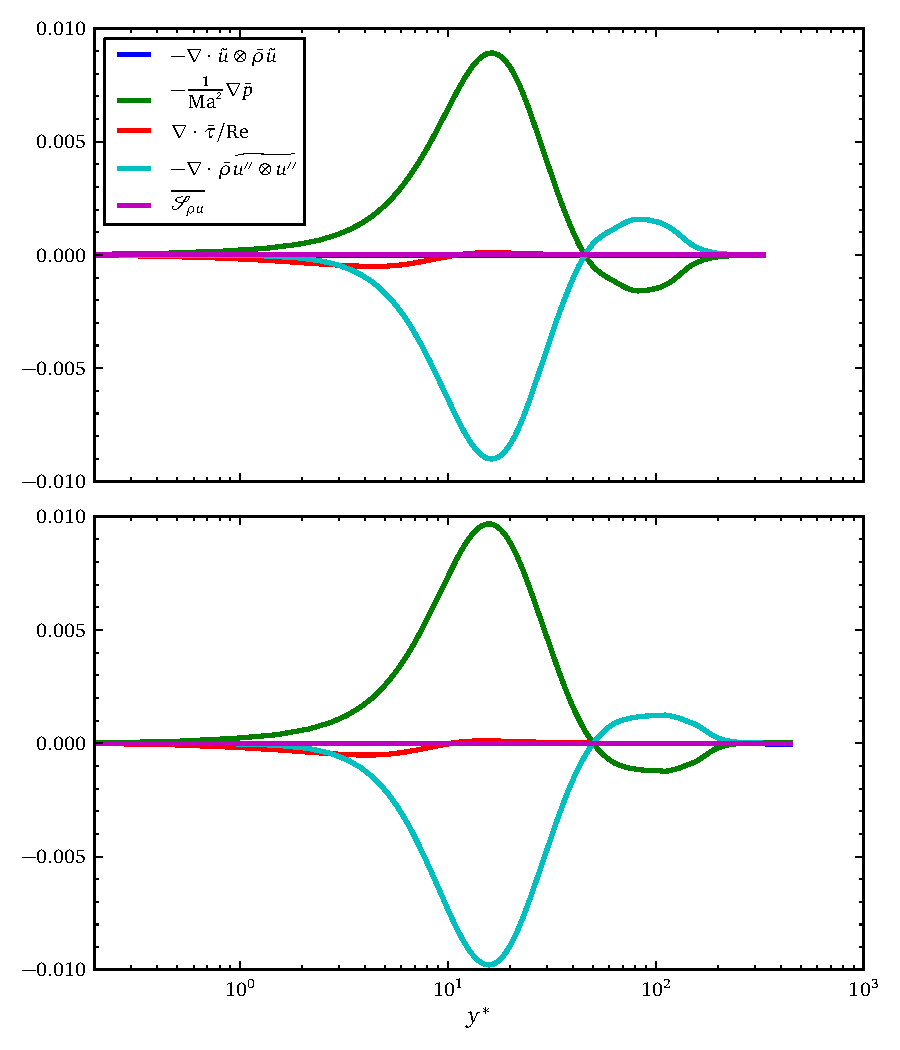
\includegraphics[width=\textwidth]{hqd_fans_rho_v}
\caption[Wall-normal momentum equation budget for cases t3.199 and t4.134]{%
    Budget for the Favre-averaged wall-normal momentum~\eqref{eq:fans_mom}
    in simulations t3.199 (above) and t4.134 (below)
    normalized by $\rho_w u_\tau^3 / \nu_w$.\label{fig:fans_rho_v}
    % Normalize by \rho_w (\partial_y u)_w u_\tau with u_tau having units u_0
}
\end{figure}

%% Spanwise momentum is zero by symmetry so this plot is just statistical noise
%\begin{figure}
%\centering
%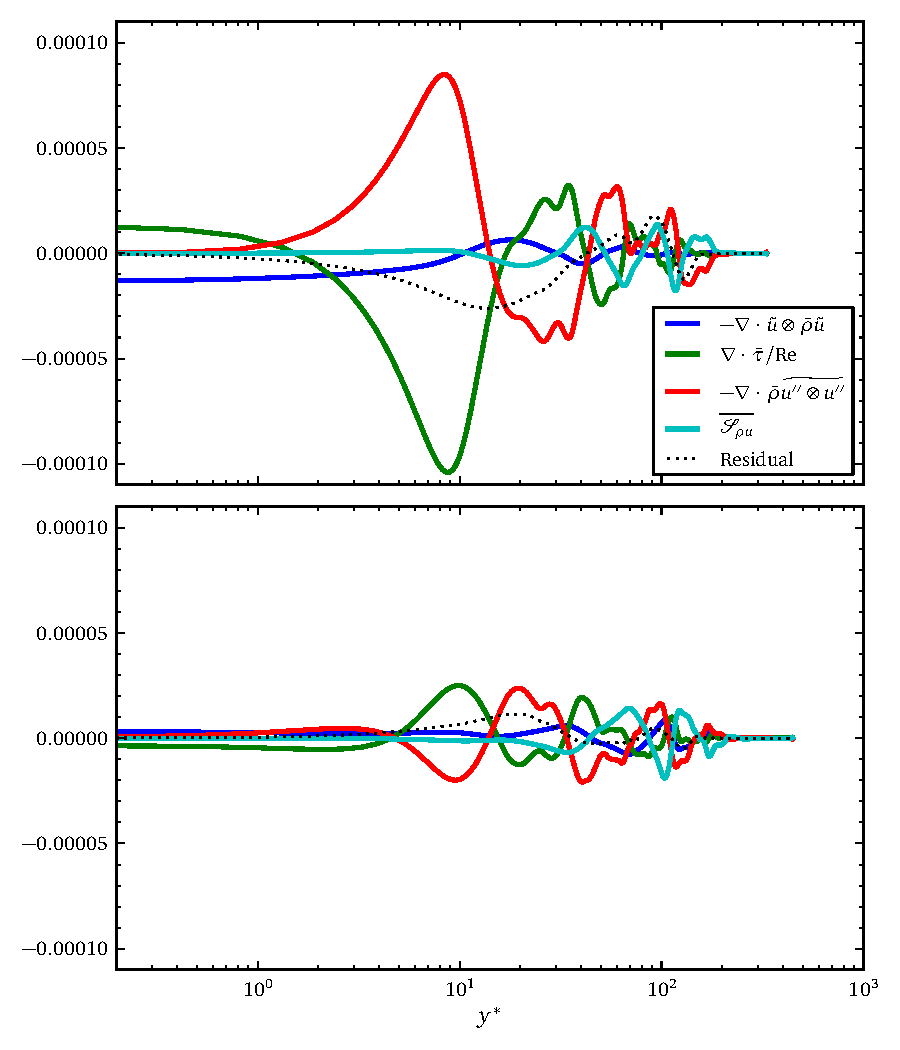
\includegraphics[width=\textwidth]{hqd_fans_rho_w}
%\caption[Spanwise momentum equation budget for cases t3.199 and t4.134]{%
%    Budget for the Favre-averaged spanwise momentum~\eqref{eq:fans_mom}
%    in simulations t3.199 (above) and t4.134 (below)
%    normalized by $\rho_w u_\tau^3 / \nu_w$.\label{fig:fans_rho_w}
%    % Normalize by \rho_w (\partial_y u)_w u_\tau with u_tau having units u_0
%}
%\end{figure}

\begin{figure}
\centering
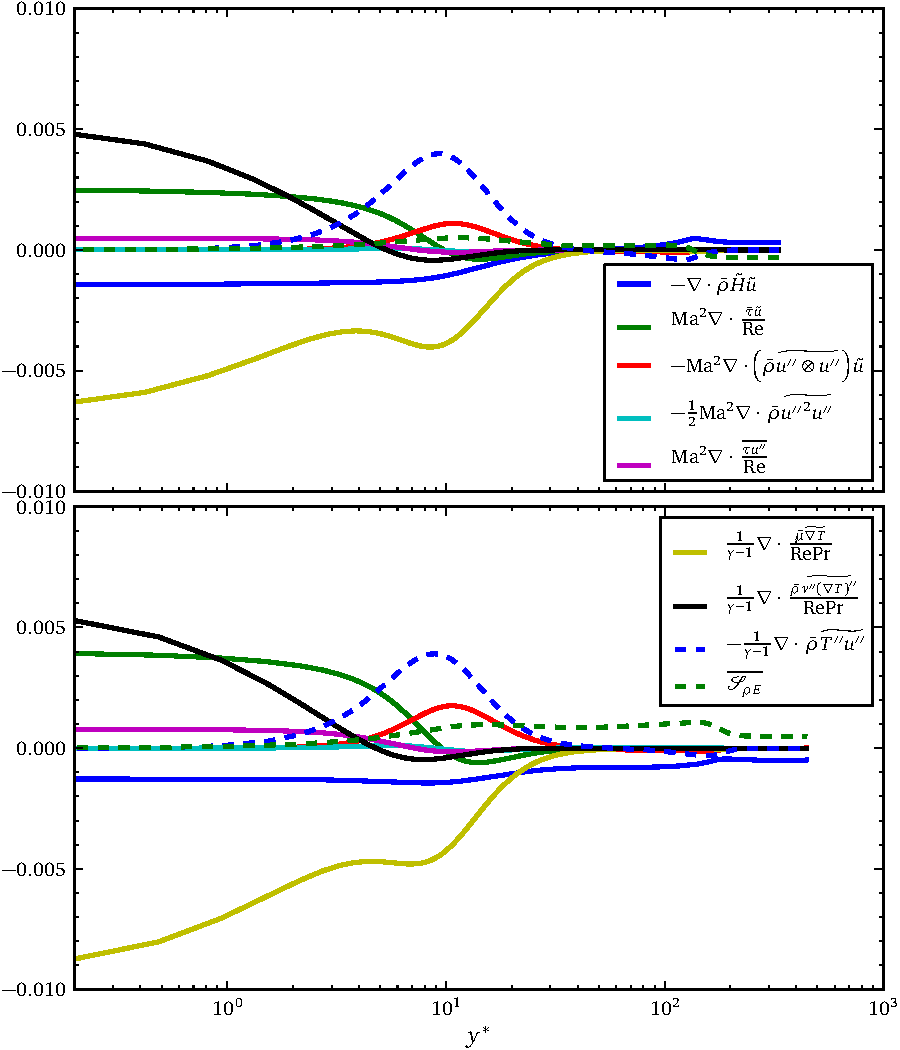
\includegraphics[width=\textwidth]{hqd_fans_rho_E}
\caption[Total energy equation budget for simulations t3.199 and t4.134]{%
    Budget for the Favre-averaged total energy~\eqref{eq:fans_energy}
    in simulations t3.199 (above) and t4.134 (below) normalized by
    $\rho_w a_w^2 u_\tau^2 / \nu_w$.\label{fig:fans_rho_E}
    % Normalize by \rho_w T_w (\partial_y u)_w
}
\end{figure}

\begin{figure}
\centering
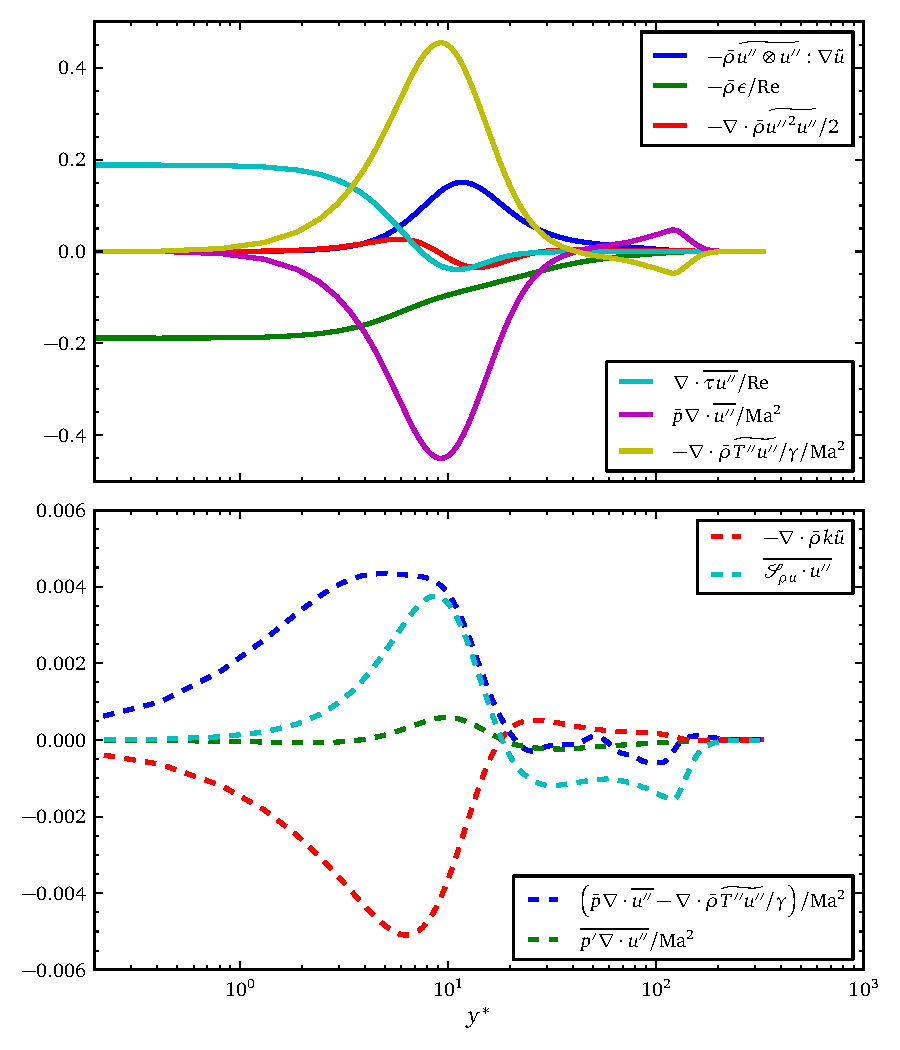
\includegraphics[width=\textwidth]{hqd_tke_t3199}
\caption[Turbulent kinetic energy equation budget for simulation t3.199]{%
    Budget for the turbulent kinetic energy~\eqref{eq:fans_tke} in simulation
    t3.199 normalized by $\rho_w u_\tau^4 / \nu_w$.  More significant terms
    appear in the upper half of the figure while less significant contributions
    appear in the lower half.  Two nearly symmetric thermodynamic terms
    above have their sum duplicated below.\label{fig:tke_t3199}
    % Normalize by \mu_w (\partial_y u)_w^{2} / Re
}
\end{figure}

\begin{figure}
\centering
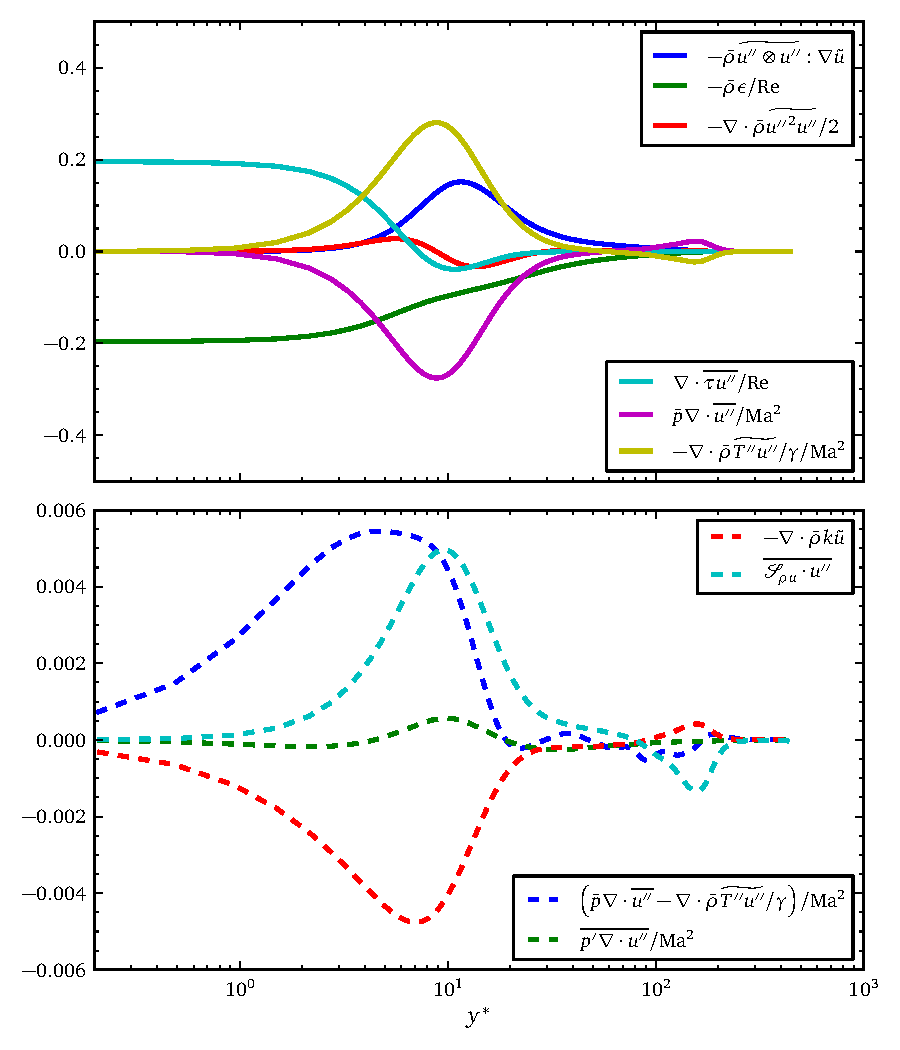
\includegraphics[width=\textwidth]{hqd_tke_t4134}
\caption[Turbulent kinetic energy equation budget for simulation t4.134]{%
    Budget for the turbulent kinetic energy~\eqref{eq:fans_tke} in simulation
    t4.134 normalized by $\rho_w u_\tau^4 / \nu_w$.  More significant terms
    appear in the upper half of the figure while less significant contributions
    appear in the lower half.  Two nearly symmetric thermodynamic terms
    above have their sum duplicated below.\label{fig:tke_t4134}
    % Normalize by \mu_w (\partial_y u)_w^{2} / Re
}
\end{figure}
